\documentclass[12pt]{article}

\usepackage[]{graphicx}
\usepackage[]{color}
\usepackage{alltt}
\usepackage{float}

\usepackage{graphicx}
\usepackage{amsmath}

\newcommand{\mytitle}{A Comparative Evaluation of the Utility of Linguistic Features for Part-of-Speech-Tagging}
\newcommand{\myname}{Marco Flöß}
\newcommand{\mysupervisor}{Prof. Dr. Christian Heumann, Dr. Matthias Assenmacher}

\usepackage[a4paper, width = 160mm, top = 35mm, bottom = 30mm, 
bindingoffset = 0mm]{geometry}
\usepackage[utf8]{inputenc}
\usepackage{ragged2e}
\usepackage{xcolor}
\usepackage[round, comma]{natbib}
\usepackage{fancyhdr}
\newcommand{\changefont}{%
    \fontsize{8}{11}\selectfont
}
\usepackage{hyperref}
\hypersetup{
  colorlinks = true,
  linkcolor = black,
  urlcolor = black,
  citecolor = black}
\pagestyle{fancy}
\fancyhead{}
\fancyhead[R]{\changefont{\mytitle}}
\fancyfoot{}
\fancyfoot[R]{\thepage}
\setlength{\headheight}{14.5pt}
\setlength{\parindent}{0pt}
\interfootnotelinepenalty = 10000

% ------------------------------------------------------------------------------
% MAIN -------------------------------------------------------------------------
% ------------------------------------------------------------------------------
\IfFileExists{upquote.sty}{\usepackage{upquote}}{}
\begin{document}

% FRONT PAGE -------------------------------------------------------------------
 
\begin{titlepage}
\begin{center}
    
\LARGE
Bachelor's Thesis
    
\vspace{0.5cm}
      
\rule{\textwidth}{1.5pt}
\LARGE
\textbf{\mytitle}
\rule{\textwidth}{1.5pt}
   
\vspace{0.5cm}
      
\large
Department of Statistics \\
Ludwig-Maximilians-Universität München 

\vfill

\Large
\textbf{\myname}

\vfill

\large
Munich, July 25\textsuperscript{th}, 2022
      
\vfill


\includegraphics[width = 0.4\textwidth]{Pictures/sigillum.png}

\vfill

\normalsize
Submitted in partial fulfillment of the requirements for the degree of B. Sc.
\\

Supervised by \mysupervisor

\end{center}
\end{titlepage}

% CONTENTS ---------------------------------------------------------------------

\pagenumbering{Roman}
\newpage

\begin{abstract}

The task of Part-of-Speech-tagging is an important step in many natural language processing tasks. It constitutes the automatic assignment of tags to words that signify their syntactic function and morphological behaviour, thereby providing valuable information which can help to disambiguate the semantic nature of the corresponding word.

This thesis explores different sources of features that can be obtained from raw text data and may prove useful to build an effective Part-of-Speech-tagging model. Therefore the word identity as a feature was encoded using dense word embeddings. The Word2Vec and FastText framework were utilized to train the respective word embeddings directly on the training data while for the GloVe framework Stanford's pre-trained word embeddings were deployed. Additionally to the word identity several groups of linguistic features were implemented regarding the kind of characters a word may encompass, the case of characters in a word, the position of a word relative to its sentence and possible affixes present in a word. 

As an architecture for the Part-of-Speech-tagger a Long-Short-Term-Memory Neural Network was chosen as it is able to capture structural regularities in sequential data and sentences are essentially sequences of words. 

The Georgetown University Multilayer Corpus constitutes the data on which all evaluations are performed and as a compilation of texts that stem from a variety of communicative purposes was deemed a reasonable basis for the analysis to generalize well to a wide scope of data. 

The utility of the before mentioned features was compared by consulting metrics such as the accuracy and weighted F1-score on the Part-of-Speech-tagging task. For models, regardless of the implemented word embedding framework, the features regarding the case of characters in a word have been shown to considerably enhance its performance across the evaluation metrics. If the GloVe framework is utilized to encode the word identity, the additional information provided by features dealing with possible affixes of words is shown to significantly improve the models performance. 

In general, this thesis first gives a theoretical introduction into the topics of Part-of-Speech-tagging, neural networks and word embeddings. 
Secondly, the practical part explores which instantiations of word embedding frameworks are favorable and afterwards compares the utility of including the different groups of linguistic features in the input for the Part-of-Speech-tagging models.

\end{abstract}

\newpage
\tableofcontents

%%%% if you would want to include material overview
%%%% use one of the following in addition
% \newpage
% \listoffigures
% \newpage
% \listoftables
\newpage

% CHAPTERS ---------------------------------------------------------------------

\pagenumbering{arabic}
    

\section{Introduction}
\label{intro}
With the advent of intelligent speech assistants such as Apple's Siri, Microsoft's Cortana and Amazon's Alexa into the daily life of numerous people, natural language processing/generation and its applications seem to have manifested themselves to stay and further shape the way humans cooperate with software. To interact with a voice-activated interface demonstrates to most users just how far the technological basis behind these applications has advanced and exhibits the capacity of algorithms to handle natural language. These bots may represent the pinnacle of current advancements to the layperson, though most of the underlying subdivisions of their software are based on tasks the fields of natural language processing, natural language generation and machine learning have been dealing with for decades. 

This thesis will have its focus on one important pre-processing task relevant to a wide variety of natural language processing applications, the automatic categorization of words in classes describing their grammatical behavior, called Part-of-Speech-tagging.

Annotating corpora with Part-of-Speech-tags has been done manually in the past \citep{martinez2012part}. One famous example of an annotated corpus, consisting of roughly one million words, is the Brown Corpus. In 1967 Henry Kucera and W. Nelson Francis compiled texts selected from a wide scope of sources of American English \citep{kucera1967brown}. This resulted in a corpus that has been cited extensively, because of its variegated nature and has been tagged partly with rule-based systems \citep{schmid1994part} and manually in the years following its compilation. Among others this annotated corpora helped to develop taggers with an accuracy of up to 97\% \citep{jurafsky2021}. Hence for the English language humans tend to perform the task of Part-of-Speech-tagging as well as the current state-of-the-art algorithms \citep{manning2011part}.

Two major difficulties for the successful completion of this task are the ambiguity of words and the encounter of before unseen words. Consider the example sentence of \cite{martinez2012part} 'We can can the can'. Three different syntactic functions of the word 'can' are represented in these five words. In order from left to right, 'can' is first an auxiliary, a verb and finally a noun, thereby showcasing the ambiguity of this word in one very short sentence.  

This thesis will first outline the general framework of Part-of-Speech-tagging. Afterwards an exploration of the theoretical foundation of LSTM (Long Short-Term Memory) Neural Networks will be given which will touch on the basic concepts of Feed-Forward and Recurrent Neural Networks as they build the foundation for the model used as the Part-of-Speech-tagger. Next a short overview will demonstrate some of the different possibilities to encode the semantic representation of a word into an embedding, thereby concluding the theoretical part of this work.

A short description of the Georgetown University Multilayer Corpus (GUM) will be provided since this annotated corpus is used for the empiric analysis. 
Following this the implementation of the feature selection process and the setup of the architecture for  the Part-of-Speech-tagging model will be examined. Finally the utility of the different linguistic features, provided as inputs to the tagger, will be evaluated.

\newpage


% Begin Theory Part 

\section{Part-of-Speech-Tagging}

\subsection{Definition}
\label{pos_def}
Part-of-Speech-tagging implements an annotation of data which proceeds at the level of words. Hereby each element of a corpus receives a morphosyntaktic label called the Part-of-Speech-tag \citep{westpfahl2020pos}. 
This label incorporates information on the morphological behaviour and syntactic function of its unit, thereby leading to the alternative naming conventions such as word classes, morphological classes or lexical tags \citep{jurafsky2021}.

In this thesis the label will always be referred to as the POS-tag. 

Since clear distinctions between these categories are an animated source of discussions, the pool of possible tags, from which a model draws, varies vehemently according to which tagset a model was trained on. These tagsets comprise categories which in unison are all-encompassing and try to provide a complete subdivision of the different morphosyntactic roles words can embody \citep{westpfahl2020pos}. 
Tagsets naturally are only applicable for one language since morphosyntactic roles vary in their delimitation between themselves and apart from that, some categories may not even have an equivalent counterpart in a language which was not the origin of the tagset.

While the decision making process for a certain POS-tag uses several features on the word itself, the process of tagging performs poorly if merely the to-be-tagged word is provided \citep{jurafsky2021}. 
The underlying algorithm of the model receives the data to be annotated sentence-wise and has access to intrinsic and extrinsic cues \citep{goldberg2017neural}. 

\subsection{Significance of accurate syntactic and lexical classification}
\label{pos_sig}
A variety of natural language processing tasks utilize the information provided by tags concerning the POS of tokens. 
While the concrete instantiation is seldom considered a relevant piece of information in the finalized output of tasks such as machine translation or information retrieval (IR), it can help to disambiguate the semantic nature of a word during parsing. 
For tokens that belong to several morphosyntactic classes inhibit an ambiguity regarding their meaning \citep{embedding2020pilehvar}.

The filtering of nouns of a corpus may provide valuable insight for the Information-Retrieval task. 

Machine translation algorithms often use POS-tags as one source of information \citep{westpfahl2020pos}.

A POS-tag is also relevant to disambiguate the cases in which varying POS-instantiations would be pronounced differently. 
The different pronunciations of 'object' come into place whether it is considered a noun or a verb where in the case of being a noun the first syllable would be stressed and in case of being a verb the second syllable.
'Content' has an emphasis on the first syllable when instantiated as a noun or on the second if considered an adjective. 

These two examples should showcase how the Part-of-Speech-tag can be relevant for producing a more accurate speech recognition system or help to choose the correct pronunciation for speech synthesis systems \citep{jurafsky2021}. 

A correct classification also provides more subtle cues considering the stem of a word or the probability of words which could appear in its vicinity.


\subsection{Tagsets}
\label{pos_tagsets}
Tagsets are compilations of the morphosyntactic roles which try to encompass a full representation of the different morphological behaviours and syntactic functions words can occupy in a certain language. 
As stated before the delimitation of these categories is not strictly defined and therefore a multitude of different tagsets has been introduced. 

Because of the ongoing discussions and the frequently indistinct boundaries of grammatical categories, tagsets aim to be pragmatic, since a pure theoretical, all-encompassing distinction of different POSs is not yet achieved and will likely not be any time soon \citep{westpfahl2020pos}. 
Additionally the slight alterations that occur constantly in natural languages impedes the realisation of a definitive discrimination.

Among the most recognized tagsets is the Brown tagset which is based on the 82 categories used on the Brown corpus. The rationale for the tagging procedure was initially introduced in \citealt{greene1971automatic}, but was extended by numerous contributors \citep{brown1979manual}. 

Another prominent tagset is CLAWS, Constituent Likelihood Automatic Word-tagging System, introduced by the Lancaster University which encompasses a varying number of different POS-tags depending on the version of its tagset. It has been continuously developed since the early 1980s \citep{garside1987claws}. Currently 8 versions are published.

The English Penn Treebank tagset consists of 36 POS-tags and 12 tags specifically for punctuation purposes. After the compilation of the roughly 4.5 million word Penn corpus by the University of Pennsylvania in 1989, it has been annotated in the following three years with its corresponding tagset \citep{marcinkiewicz1994building}.

In this thesis the tagset of the Universal Dependencies (UD) framework with its 17 tags will be used. It has become widely accepted as one of the most important tagsets, since it has treebanks for over 100 languages \citep{ud2022opencom}. It is an open community effort. The tags in it are:
\begin{description}
\item[ADJ] Adjective: noun modifiers describing properties
\item[ADV] Adverb: verb modifiers of time, place, manner
\item[NOUN] words for persons, places, things, etc.
\item[VERB] words for actions and processes
\item[PROPN] Proper noun: name of a person, organization, place, etc..
\item[INTJ] Interjection: exclamation, greeting, yes/no response, etc.
\item[ADP] Adposition (Preposition/Postposition): marks a noun’s spacial, temporal, or other relation
\item[AUX] Auxiliary: helping verb marking tense, aspect, mood, etc.
\item[CCONJ] Coordinating Conjunction: joins two phrases/clauses
\item[DET] Determiner: marks noun phrase properties
\item[NUM] Numeral
\item[PART] Particle: a preposition-like form used together with a verb
\item[PRON] Pronoun: a shorthand for referring to an entity or event
\item[SCONJ] Subordinating Conjunction: joins a main clause with a
subordinate clause such as a sentential complement
\item[PUNCT] Punctuation
\item[SYM] Symbols like \$ or emoji
\item[X] Other
\end{description}
















\subsection{Related linguistic features}
\label{pos_features}
\cite{goldberg2017neural} divides the sources of information for POS-tagging into two major groups. 
One is formed by the utilization of attributes of the word itself which from now on will be called intrinsic cues. 
These stand against the complementary group of extrinsic cues that compromise all features the context of the to be tagged word, the sentence, is able to provide.

As mentioned before POS-tags hold information on the morphosyntactic nature of a word. 
Therefore the the inverse direction, morphological and syntactic attributes provide information on the respective POS-tag, may hold valuable data, too.

Intrinsic cues unsurprisingly are based mostly on the morphological characteristic of a token. 
Depending on the level of inflection present in a language, the morphology of a word can be indicative of its syntactic function \citep{earl1966part}. 
In comparison to other languages, English is not a highly inflected language though in many cases a relationship between form and POS-tag is present.
For example the suffix '-ed' is, with a high probability, an indication for a past-tense verb, just as the prefix 'un-' will be incorporated at the beginning of an adjective most of the time.
Another important intrinsic cue for POS-tagging is the identity of the word itself which in an unambiguous language would be sufficient to build an infallible tagger, but even in ambiguous settings the identity is linked to a certain probability distribution for its tag \citep{goldberg2017neural}. 
Finally sub-word information such as the incorporation of capital or non-alphanumeric characters and digits may be used as features for POS-tagging.

On the other hand extrinsic cues are based on all information which can be gathered without considering the target word for the current decision.
While we may not have direct information on the syntactic function of a word in an untagged sentence, the position in the sentence in relationship to the other words is to be considered an indication of its syntactic role. 
Therefore it is paramount to consider the surrounding words and their features to make an prediction for the target word. 
Additionally to the intrinsic cues we obtained for each preceding word, the predicted POS-tag for these tokens in the sentence may be beneficial, provided that we make the tagging decision sequentially \citep{goldberg2017neural}.




\section{Neural Networks}

\subsection{The modeling of the logical XOR}
\label{nn_xor}
While for many problem cases linear classifiers perform reasonable well, 
the restriction that purely linear decision boundaries for the classification can be modeled limit their scope of application.

This restriction was prominently demonstrated by \citet{MinskyPerceptrons}. They illustrated that for the different input combinations to the logical XOR operator, no linear decision boundary could be perceived for its outputs. A simple neural network may solve this problem. 
In the following section the boolean values True and False will be interchangeably used with their respective numeric representations 1 (True) and 0 (False).

The XOR operator is true if and only if one of two logical values on which this operator is used is true.

\begin{figure}[H]
  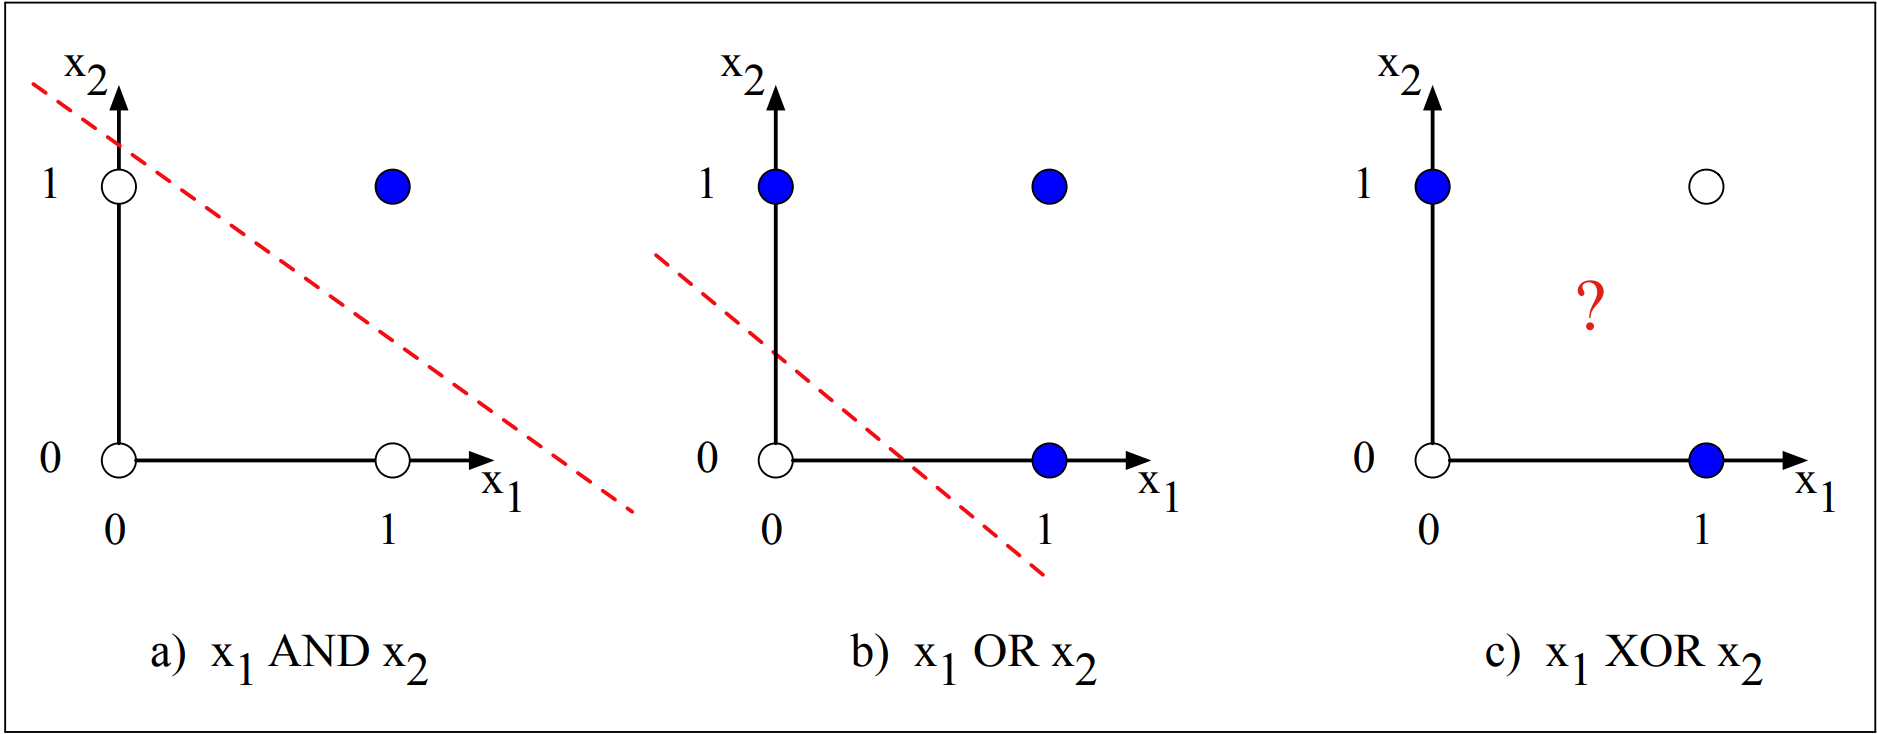
\includegraphics[width=\linewidth]{Pictures/Jurafsky_21_XOR_1.png}
  \caption{Adapted from \citet{jurafsky2021}: Visualisation of the logical functions a) AND, b) OR and c) XOR in a two dimensional space. If the points are blue the logical operator is True for this combination of truth values.}
  \label{fig:XOR1}
\end{figure}

In figure \ref{fig:XOR1}  three basic logical operators are shown in two-dimensional space where each axis represents the value of the boolean variables called $x_1, x_2$ respectively.
For the logical AND and OR one can easily assess that a linear decision boundary is conceivable. 
For the logical XOR on the other hand no decision boundary to separate the resulting boolean values can be reached in such a way.

Here the concept of layering multiple layers of processing units and applying non-linear functions on them can solve this. 
By adding a hidden layer the input values change eventually into a representation that is more favorable for basing a decision on.

\begin{figure}
  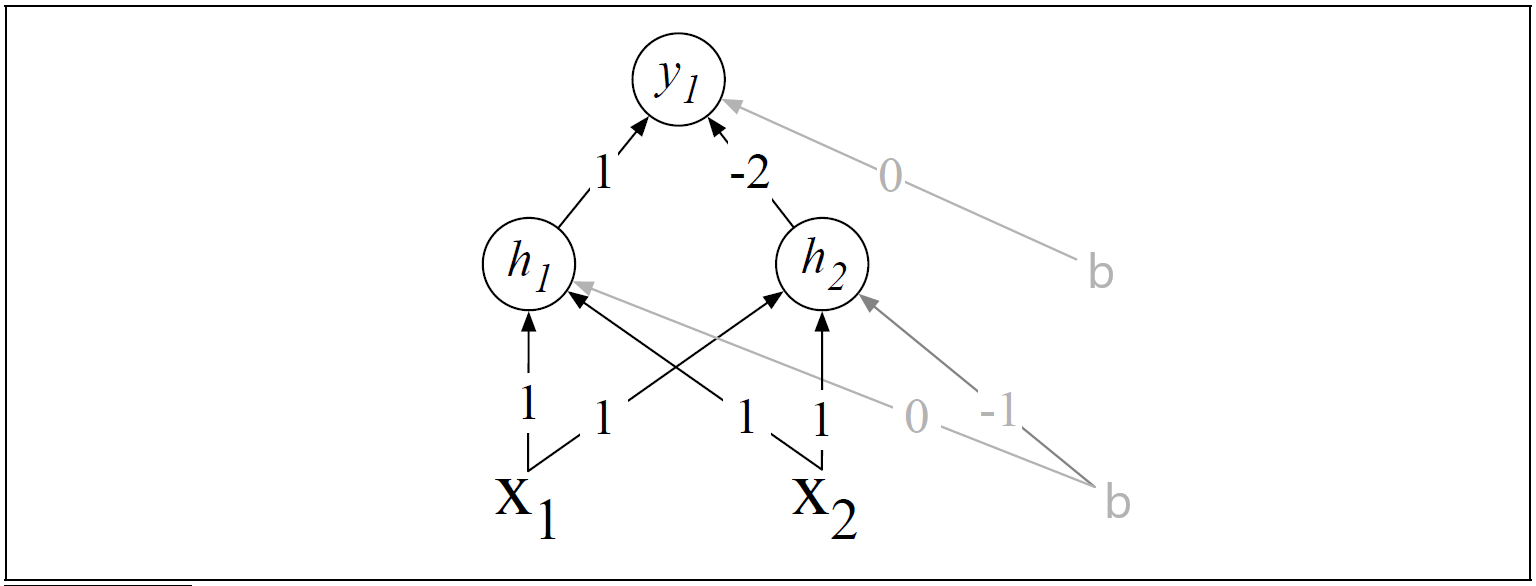
\includegraphics[width=\linewidth]{Pictures/Jurafsky_21_XOR_2.png}
  \caption{Adapted and modified from \citet{jurafsky2021}: Two-layer neural network to model the XOR operator}
  \label{fig:XOR2}
\end{figure}


Figure \ref{fig:XOR2} shows the processing units by circles with h inside for the hidden units and y for the output unit.
Weights are depicted by numbers on the black arrows and the value of the bias b for a unit by the number on a grey arrow.
Each unit multiplies the incoming values with the weights, sums them up, adds the bias and then returns the value if it is greater than 0, else 0 is given as its output. 
This filtering of outputs on whether the value is at least 0 is known as using the Rectified Linear Unit ($ReLU$) activation function which will be explored in more detail in \ref{nn_act}.

To give one example, in the case that both input variables $x_1,x_2$ are true, the input for this network is [1,1]. 
The computation that happens in $h_1$ is summing up $x_1$ times the weight from $x_1$ to $h_1$ (1*1), $x_2$ times the weight from $x_2$ to $h_1$ (1*1) and 
the bias that goes to $h_1$ (0) and afterwards returning 2 since this value is bigger than 0. 
In the second hidden node the computation happens similarly and its return value is 1. 
Therefore the input for the last layer which consists of only one unit $y_1$ which is called the output layer is [2,1]. 
Once the computation is finished for the last layer the return value is 0 which is the correct value in this case for the XOR operator. 

\begin{figure}
  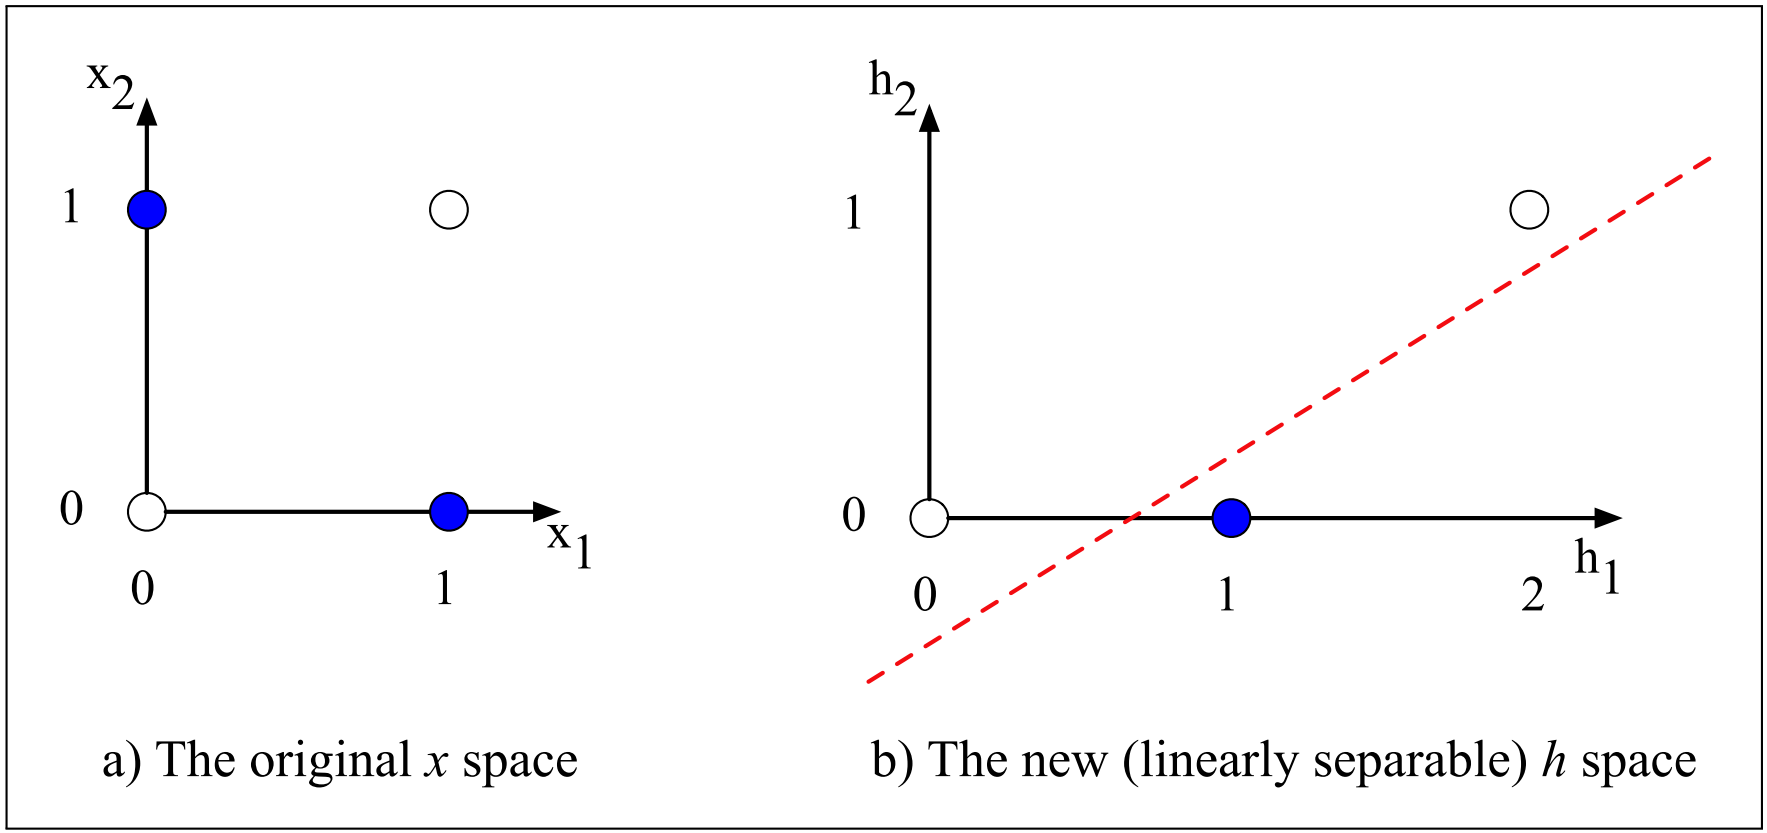
\includegraphics[width=\linewidth]{Pictures/Jurafsky_21_XOR_3.png}
  \caption{Adapted from \citet{jurafsky2021}: All cases for inputs to the XOR operator: a) are shown in their original configuration. b) have been transformed by passing the hidden layer (h) shown in Figure \ref{fig:XOR2}}
  \label{fig:XOR3}
\end{figure}

This can be done for all input combinations and it will return the appropriate value the XOR operator should return. 

After passing the hidden layer the input has been transformed into a different kind of representation of the data it held. 
If one computes the values of the hidden layer for all input combinations, the new resulting representation is linearly separable. 
Cases for which the XOR operator should return True have collapsed into the representation of [0,1] where the first value represents the first hidden unit's output and the second the other one. 
Figure \ref{fig:XOR3} shows the representation of data after the hidden layer for all cases. 
In b) we can now conceive a linear decision boundary which was not possible beforehand.



\subsection{Feed-Forward Neural Networks}
\label{nn_ff}
While the last chapter has shown the application of a neural network for a simple use case, 
this chapter will go into more detail on the different parts of such a model and its configuration.

The fact that this model incorporates numerous processing units that compute a single output which is passed on to other units was inspired by the brain's computational mechanism, 
though to compare it to the real neural system in human brains makes an overly simplistic assumption on our cognitive system and is not accurate and just the naming convention has stuck \citep{goldberg2017neural}.

In general a neural network takes input values in form of numeric vectors.
In this thesis a single input vector will be notated by $x$. 
The training of such a model takes not one input vector at a time, but rather a so called batch which is the collection of a certain number of input vectors into a matrix where the rows represent the different samples. 
To reference the j-th value of the i-th sample in the input matrix the notation is $\textbf{X}_{i,j}$.

Next it has any number of layers which consist of an arbitrary number of processing units. 
All layers that are not the input vector or the last layer in line are called hidden layers since during computations the user does not interact with them. 
These will be referred to as $h^{(k)}$ where it is the k-th hidden layer.

Finally the layer which produces the output of the whole model is called output layer which is notated by $y$. 

If all the units between two layers are connected to each other, the network is called fully connected or affine \citep{goldberg2017neural}.

All the units take as input the outputs of connected units of the layer before, multiply them with weights $\textbf{W}$ which are specific for this layer and in most cases sum up the results of the multiplication. 
Seldom, instead of summing up the results of the multiplications, a unit could just use the maximum or some other statistics on them \citep{goldberg2017neural}.

Once this step is done the unit adds a bias $b$ and applies a non-linear function which will produce the output that will be passed on to the next layer. 
Without separating these linear combinations by these so called activation functions the whole neural network would be a long, but linear function of the input values itself. 

Activation functions transform the value as the last step of all processes done by a unit and in many cases scale its output. 

Suppose we have a batch of 100 samples with a length of their input of 20, one hidden layer with 30 units and the output layer with 10 units. Then we have the following matrices and vectors with their dimensionality:
 
\[    \textbf{X} \in {\rm I\!R}^{100 \times 20}  \]
\[    \textbf{X}_{1 .} = x^{(1)} \in {\rm I\!R}^{20}  \]
\[    \textbf{W}^{(1)} \in {\rm I\!R}^{20 \times 30}  \] 
\[    b^{(1)} \in {\rm I\!R}^{30}  \]
\[    h^{(1)} \in {\rm I\!R}^{30}  \]
\[    \textbf{W}^{(2)} \in {\rm I\!R}^{30 \times 10}  \]
\[    b^{(2)} \in {\rm I\!R}^{10}  \]
\[    y \in {\rm I\!R}^{10}  \]

If we consider a single input sample, vector $x$, we can associate the units of layers with the scalar values they return for their singular (not a batch/matrix) input and the dimensionality seen above stays correct. 
For simplicity activation functions are represented by the lower case letter 'a' and are not yet specified in more detail, but could be any function presented in \ref{nn_act}. 

\[   h^{(1)} = a_1(x\textbf{W}^{(1)} + b^{(1)})   \]
\[   y = a_2(h^{(1)} \textbf{W} + b^{(2)})   \]

If the whole batch of samples is propagated through this example neural network, the whole equation would be:

\begin{equation} 
\label{eq:1}
    a_2(a_1(\textbf{X}\textbf{W}^{(1)} + \textbf{b}^{(1)}) \textbf{W}^{(2)} + \textbf{b}^{(2)})
\end{equation}

This would result into an output with the dimensionality of $100 \times 10$ where each row represents the output of layer $y$ for one row of the input matrix \textbf{X}. In the equation with matrices the bias vectors $b^{(k)}$ are added similarly for each row of the matrix to the left side of the addition sign or can just be considered as a matrix with the same bias vector for all its rows.

Considering \textbf{X} as the beginning of the information flow through the neural network, it is first passed on through the hidden layer $h^{(1)}$ and finally through the output layer $y$. The direction of the information flow is merely forward through the different layers which motivated the naming convention for such simple models as Feed-Forward Neural Network. The flow of information can be passed back to previous layers for Recurrent Neural Network which will be defined in \ref{nn_rnn}.

In the following section four of the most important activation functions are presented.


%-------------------------------------------------------------------------------------------


\subsubsection{Activation functions}
\label{nn_act}

First of is the sigmoid $\sigma$ function, shown in equation \ref{eq:simoid}, which maps any value it receives onto the range [0,1], a property that makes this activation function attractive for the usage at an output layer where a probability for binary classification is considered useful. Additionally the effect of outliers for possible following layers is mitigated.

\begin{equation}
\label{eq:simoid}
    \sigma(x) = 1 / (1 + e^{-x})
\end{equation}


Next of is the hyperbolic tangent $tanh$ function which behaves very similarly to the sigmoid function except that it squashes the values to the range of [-1,1] and thereby maps outliers towards the mean \citep{jurafsky2021}. Its equation is the following:

\begin{equation}
\label{eq:tanh}
    tanh(x) = (e^x - e^{-x}) / (e^x + e^{-x}) 
\end{equation}

It's derivative is vanishing less quickly than the sigmoid's which is a favorable property for the training process explained in \ref{nn_train}.


Build as an approximation of the $tanh$ activation function the hard tanh $hardtanh$, shown in equation \ref{eq:htanh}, is a more computationally efficient alternative \citep{goldberg2017neural}.
    
\begin{equation}
\label{eq:htanh}
    hardtanh(x) = \begin{cases}
  -1   \text{\phantom{xx} x $<$ -1} \\
   1   \text{\phantom{xxxi} x $>$ 1} \\
   0   \text{\phantom{xxxi} otherwise.}
\end{cases}
\end{equation}
    


Finally, the Rectified Linear Unit $ReLU$ activation function which we have already seen in chapter \ref{nn_xor} is presented. 
Positive values given to this function will be returned without any modification and negative values are capped so that the smallest value this function returns is 0. This can be mathematically expressed as in equation \ref{eq:relu}. 
$ReLU$ is computationally very efficient and has nearly linear properties \citep{jurafsky2021}. 

\begin{equation}
\label{eq:relu}
    ReLU(x) = max(0, x)
\end{equation}

It's derivative is either 0 for all values less than zero or 1 for all values greater than zero. 
The property that the gradient for positive values is constantly at 1 is one advantage of $ReLU$ over the other activation functions presented here since the other functions struggle with the fact that their gradients may become infinitesimal small or are 0 for extreme values.

In figure \ref{fig:AF} the four activation functions are plotted and their respective derivatives.

\begin{figure}
  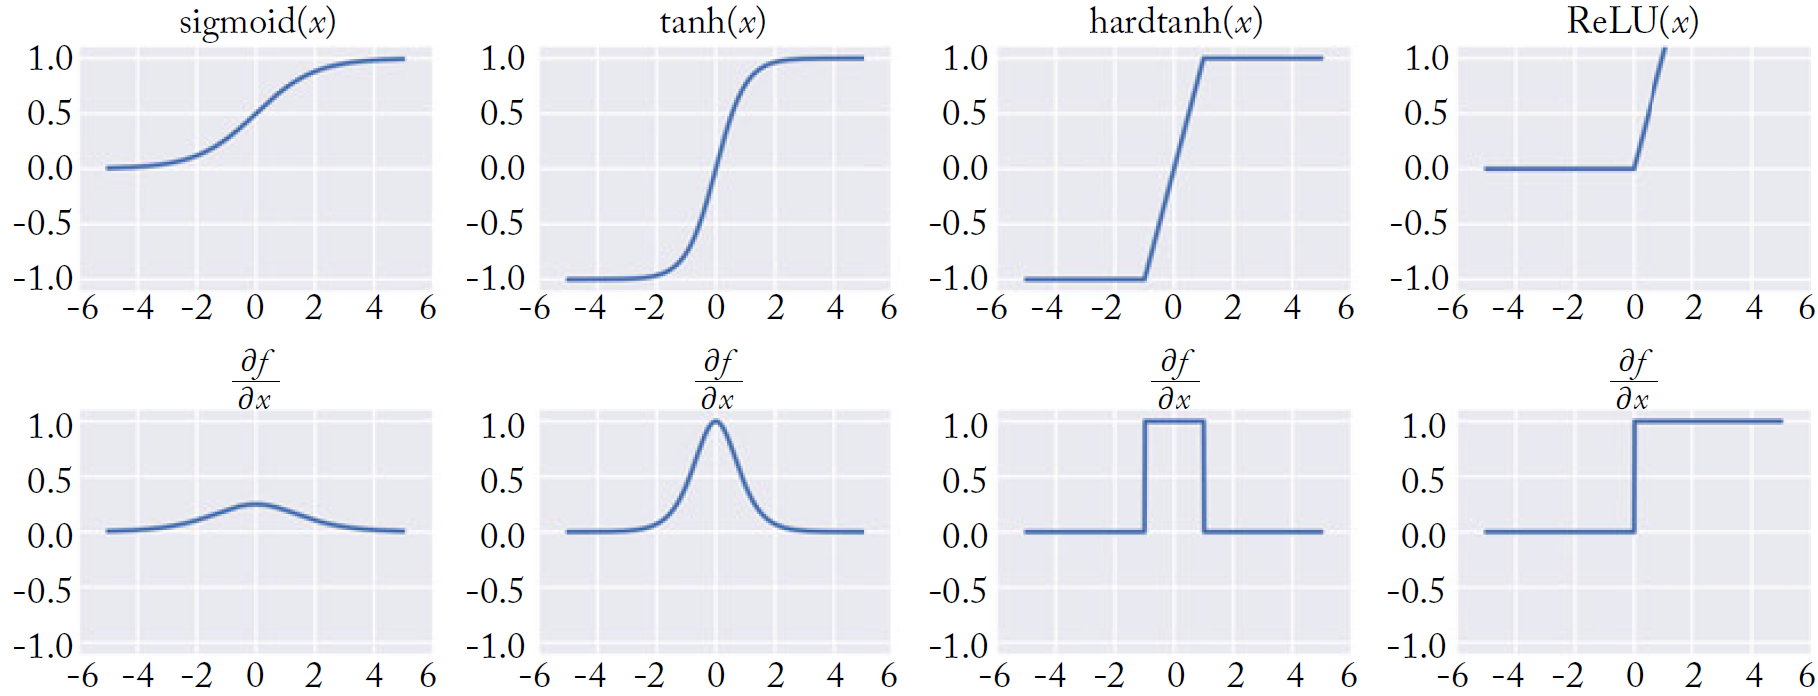
\includegraphics[width=\linewidth]{Pictures/Goldberg_17_AF.png}
  \caption{Adapted from \citet{goldberg2017neural}: Plots of the functions and their derivatives for the sigmoid, tanh, hardtanh and ReLU activation function}
  \label{fig:AF}
\end{figure}

While not strictly speaking an activation function, it's application on whole vectors of output layers make the $softmax$, shown in equation \ref{eq:softmax}, somewhat related to the functions mentioned above. 

\begin{equation}
\label{eq:softmax}
    softmax(x_i) = e^x_i / \sum_{j=1}^{C} e^{x_j}
\end{equation}

For the output layer in settings where a probability distribution over different class choices is favorable, e.g. POS-tagging, the $softmax$ function is used on the units of the output layer. 
It normalize all the values in such a way that their sum is 1 and they can be regarded as conditional probabilities for being a certain class \citep{jurafsky2021}.

In Equation \ref{eq:softmax} we suppose that the final layer has C units.


%-------------------------------------------------------------------------------------------


\subsubsection{Loss function}
As neural networks are an instance of supervised machine learning, we possess the correct output for the samples on which we train our model. 

To extract information on the model's quality on performing a certain task, we need to quantify the degree to which the model makes the right decisions. 
Therefore a so called loss function is instantiated which compares the model's output with the validated output we have on our training data and applies different metrics to make the correctness tangible.
Since the neural network usually provides a distribution as its output for a given prediction, conditioned on the input it has received and the model's parameters, the final decision is based on the principle of maximum likelihood \citep{jurafsky2021}.

This limits the scope of this thesis and its the application of the described neural networks to tasks where there is one correct output among at least two choices.
This makes the Cross-Entropy ($L_{CE}$) loss function, as seen in equation \ref{eq:cross}, a valid choice to quantify the distance between the model's decisions and the gold standard \citep{Goodfellow-et-al-2016}.

\begin{equation}
\label{eq:cross}
    L_{CE}(\hat{y},y) = \sum_{i=1}^{C} y_i log\hat{y}_i
\end{equation}

In this equation we suppose that our output is a vector of length $C$ which represents the number of possible categories from which the model has to choose. 
The gold standard that was not generated by the model is a one-hot-encoded vector in which the true class is encoded as 1, while the other positions in the vector are 0.

In cases in which we use the neural network for a binary classification task the Cross-Entropy loss function can be reduced to a function which is analogous to the loss function for a logistic regression \citep{jurafsky2021}.

One alternative loss function, though mostly used in linear regression tasks, would be the Mean Squared Error loss (MSE). It sums up the squared distances between the model's prediction and the real output for each possible class. Afterwards it is multiplied by the inverse of the number of classes ($C$) as shown in equation \ref{eq:mse}:

\begin{equation}
\label{eq:mse}
    L_{MSE}(\hat{y},y) = (1/C) * \sum_{i=1}^{C} (y_i - \hat{y}_i)^2
\end{equation}

The MSE is seldom a reasonable choice for classification tasks in neural networks. The fact that the usage of this loss function assumes the data to be derived from a normal distribution and the assumption that the values provided to the function are arbitrary real valued numbers, not restricted to the range of probabilities [0,1], makes the MSE inappropriate for most settings for which neural networks are used \citep{khan2019mse}.


%-------------------------------------------------------------------------------------------


\subsubsection{Training Neural Networks}
\label{nn_train}
So once a loss function is chosen, input data, typically in batches, can be fed into the neural network and it will pass through the consecutive layers and produce an output. 
Afterwards the loss is calculated for the model and it is possible to quantify the distance between the correct output and the predicted one. 
This flow of data through all the computations is called the forward pass \citep{goldberg2017neural}.

We can use the information the loss function provides to adjust the weights and biases, the parameters, of the model and ideally make it perform better. 
This is done by minimizing the loss and computing the partial derivatives of the loss function with respect to each parameter of the neural network and adjusting the parameters according to them \citep{Goodfellow-et-al-2016}.

Even if the loss function itself is not necessarily convex which means that there might be local minima in which the optimization might get stuck, gradient based methods like gradient descent for training a neural network are widely used and have proven to work well in practice \citep{goldberg2017neural}.

Since the model consists of several layers with a multitude of parameters each, the task of calculating the gradient can get very complex and cumbersome. 
Therefore the chain-rule of differentiation is applied to make the calculations more docile.

Often computation graphs, which are directed acyclic graphs of the partial calculations involved in computing the loss, are used to simplify the process of determining the gradient and derivatives for the model \citep{goldberg2017neural}.
Being broken down into separate operations the forward pass through the neural network will produce some additional intermediate results, but its major gain lies in the backward pass of information.

By using the chain-rule a gradient for each operation in the computation graph can be computed step by step through the directed acyclic graph by using the gradient gotten from the previous step.

The name backward pass springs from the fact that the first derivative we compute starts at the loss function itself and we move backwards through all the operations involved. This procedure is called the error backpropagation algorithm \citep{jurafsky2021}.

Since the forward pass has produced the intermediate results for all operations in the chain of equations, the derivatives are easily calculated once the partial gradients are worked out \citep{jurafsky2021}.

Afterwards these are used to adjust weights and biases of the model after being multiplied with a learning rate which tries to stabilize the training process.




\subsection{Recurrent Neural Networks}
\label{nn_rnn}
For applications in which the input-output mapping is static, Feed-Forward Neural Networks suffice most of the time.
As soon as temporal correlations between the samples exists, this static assumption becomes inadequate \citep{tsoi1997recurrent}. 
Temporal correlation can mean that the input instances happened sequentially or that an order persists between them. 
Feed-Forward Neural Networks do not incorporate these structural properties of the input which may hold valuable information for task in which the sequential nature of data is of relevance.

Therefore the concept of Recurrent Neural Networks (RNN) is introduced for sequences of inputs and the ability to capture statistical regularities in them \citep{goldberg2017neural}.

These regularities are captured by the fact that previous inputs may influence the current information flow by a recurrent state element specific to RNNs. 
So the flow of information is not only forward, but has a cyclic element to it \citep{jurafsky2021}. 
Incorporating such feedback loops allows the neural network to exhibit a temporal dynamic behaviour and, as \citet{embedding2020pilehvar} puts it, remember the past. 
In figure \ref{fig:RNN_1} this is exemplified by the connection of the same unit in the model with itself at the time the next input instance is fed through it.

\begin{figure}
  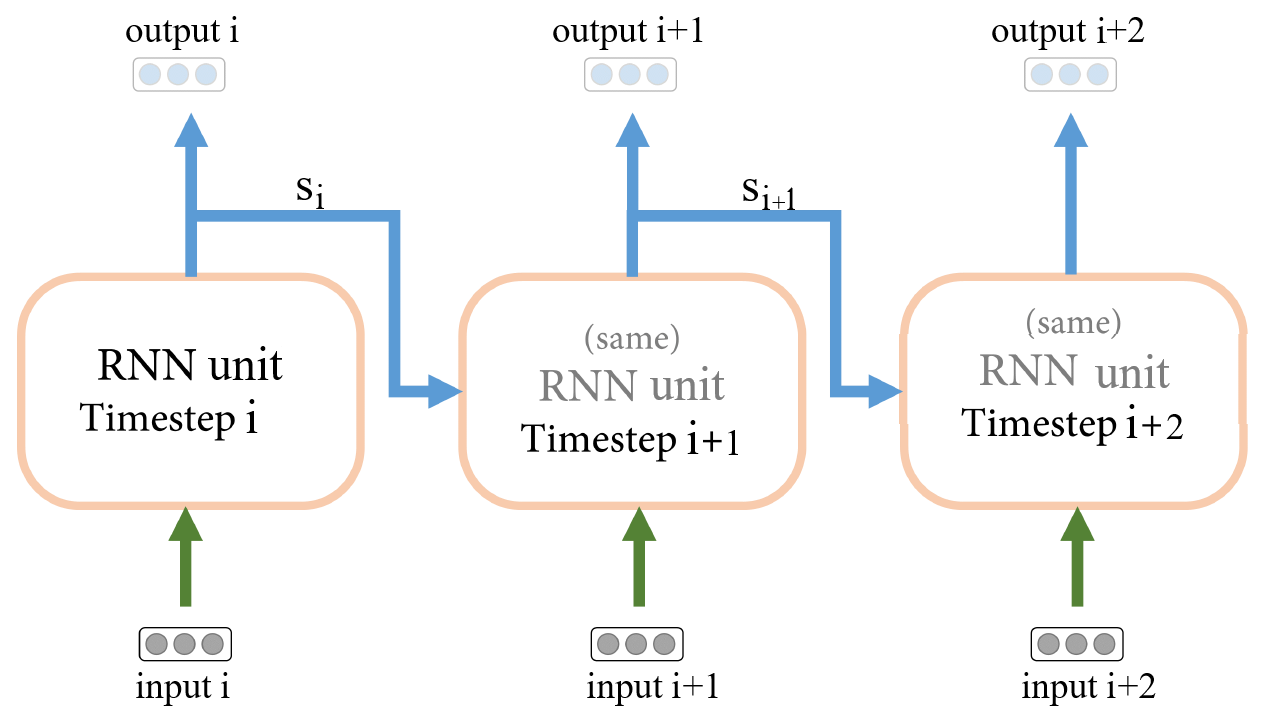
\includegraphics[width=\linewidth]{Pictures/Pilehvar_20_RNN.png}
  \caption{Adapted and modified from \citet{embedding2020pilehvar}: Visualization of a single unit of a RNN for sequential data. These three time correlated or sequential instances $i, i+1, i+2$ show the recurrence of the model by the two arrows between the unit in different time steps.}
  \label{fig:RNN_1}
\end{figure}


On a mathematical level this is achieved by making a prediction at point $i$ in a sequence dependent on all inputs up to index $i$ in the sequence, $x_{1:i-1}$. 
In general terms this can be represented, without specifying a concrete model architecture, by a recursive state element $s$. 
It incorporates the information of previous time steps and is combined with the current input to generate the recursive state element for the current prediction and for providing memory for the next time step.

\begin{equation}
\label{eq:R}
    s_i = R(s_{i-1}, x_i)
\end{equation}

In equation \ref{eq:R} the letter 'R' is used as a placeholder for a multitude of recursive techniques for which the model architectures may incorporate the information of former states. In case of the first input vector the previous recursive state element $s$ is a zero vector.
A concrete implementation of $s$ will be given in more detail for the architecture of LSTM Neural Networks in \ref{nn_lstm}.

One major difficulty when training Neural Network occurs due to the so called vanishing gradient problem. 
As explained in \ref{nn_train} the adjustment of weights and biases of the model happens according to the calculated gradients and derivatives starting at the loss and propagating backwards.
Since the calculation of gradients uses the results of the preceding steps in the backwards pass through the broken down equations of the whole model, 
the values of the gradients may vanish or, in cases of activation functions not presented here, explode when put through the activation functions used on the layers \citep{embedding2020pilehvar}.

If one considers the gradients of activation functions presented in figure \ref{fig:AF} one can assess that their gradients are in the range of values between 0 to 1. 
As their gradients become close to 0 and the backpropagation multiplies these low values several times, the resulting gradients may get vanishingly low \citep{tsoi1997recurrent}.

This problem especially arises for Recurrent Neural Networks since it incorporates a recursive element in the model to capture the structural properties of the input data.
Therefore an increasing number of multiplications with very low values may take place once the error backpropagation has passed through some recurrences. 
Consequently the adjustments of the according parameters happens only at a vanishingly low rate that makes the training procedure very inefficient. 
The problem of inefficiently capturing long-range dependencies was thoroughly investigated by \citet{gradient1994bengio}.

Another difficulty these models deal with is the fact that the recurrent state element \textbf{s} has to provide relevant information for the current decision while at the same time try to retain information for future decisions. 

One way to deal with these problems is to use gated varients of Recurrent Neural Networks.




\subsection{Long-Short-Term-Memory Neural Networks}
\label{nn_lstm}
One widely used variant to deal with the before mentioned problems for Recurrent Neural Networks are LSTMs. 
These so called Long-Short-Term-Memory (LSTM) Neural Networks split the two tasks the recurrent state element \textbf{s} in basic Recurrent Neural Networks has into two layers present in each processing unit which are controlled by gates. 
Therefore these models are considered gated-architectures and the accessed memory is regulated and so is its output \citep{goldberg2017neural}.

A LSTM Neural Network unit incorporates a context layer $c$ which tries to capture the information relevant for future predictions while forgetting some of its past information. 
This layer is regulated by the forget gate and the input gate.

Additionally, the units possess a hidden state $h$ layer that gets updated by the current context state and this update is regulated by the so called output gate. Since the context state captures structural information relevant for future predictions, the hidden state can capitalize on the task of encompassing the most valuable information for the current prediction \citep{jurafsky2021}.

These additional internal mechanisms, called gates, in combination with the additional context layer are integrated to, as  \citet{embedding2020pilehvar} puts it, make the memory last longer.


\begin{figure}
    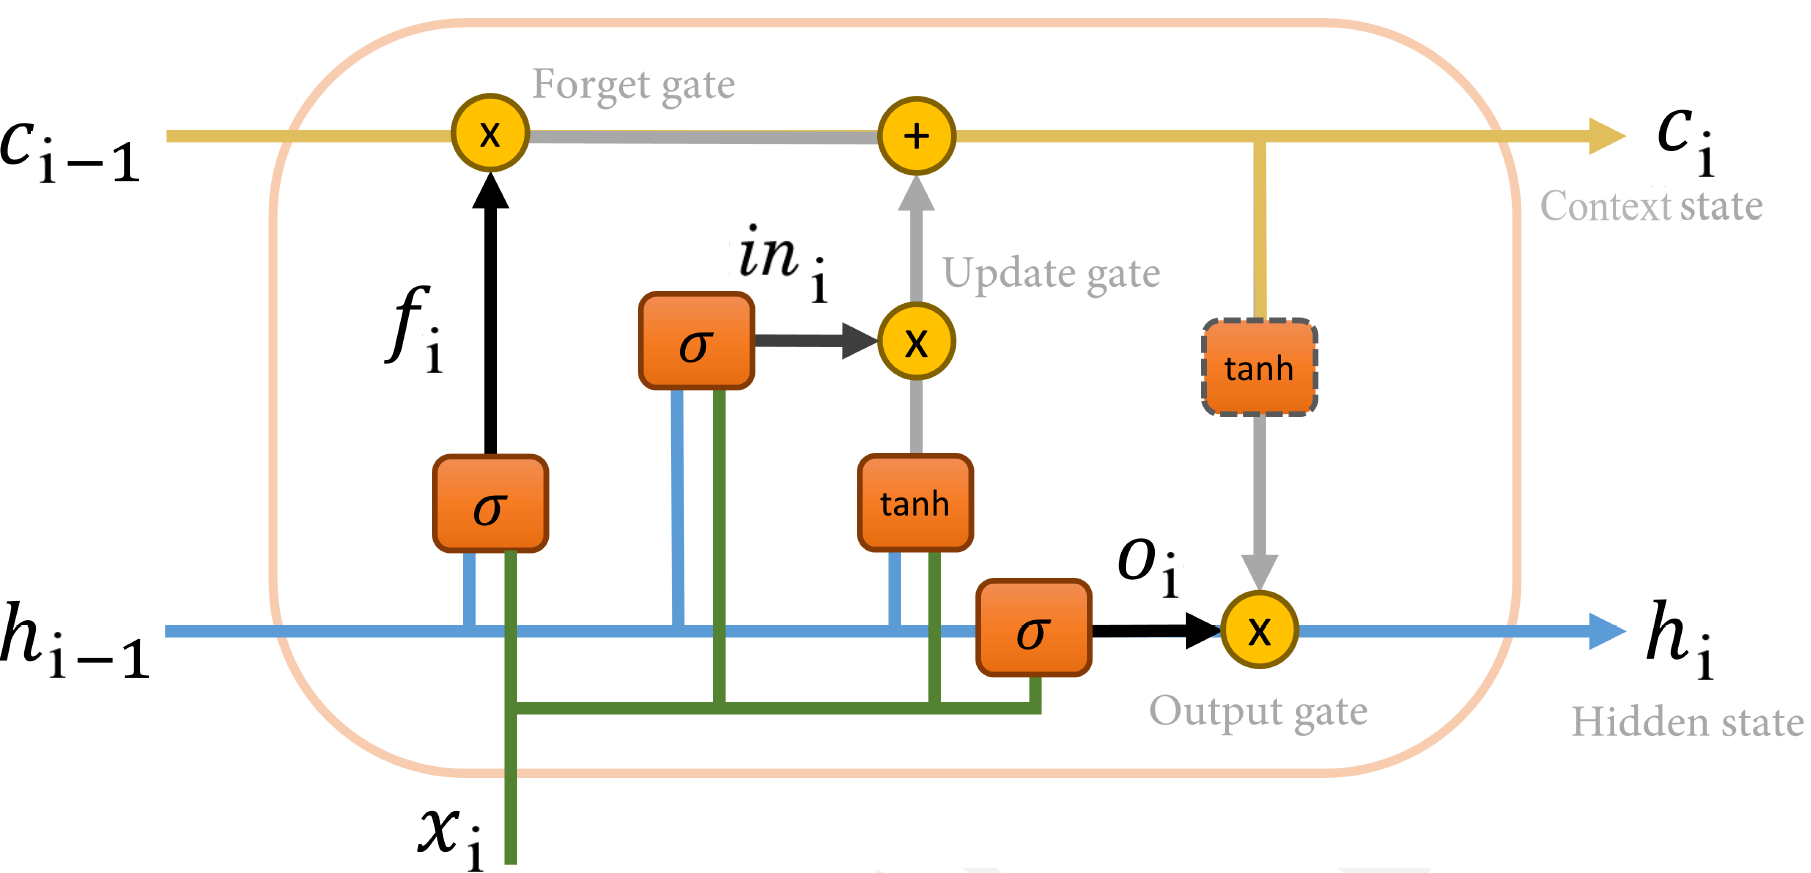
\includegraphics[width=\linewidth]{Pictures/Pilehvar_20_LSTM.png}
    \caption{Adapted and modified from \citet{embedding2020pilehvar}: Visualization of a processing unit in a LSTM. It receives the previous hidden state $h_{i-1}$, the previous context state $c_{i-1}$, the current input vector $x_i$} and produces as outputs the hidden state $h_i$ and context state $c_i$ for the current step in the sequence. The forget gate $f_i$, the input gate $in_i$ and the output gate $o_i$ are the controlling mechanisms to regulate the information flow between its inputs and outputs.
    \label{fig:LSTM}
\end{figure}

In figure \ref{fig:LSTM} the installation of an unit in a LSTM is visualised. Each unit gets fed the current input $x_i$ along with the hidden state $h_{i-1}$ and the context state $c_{i-1}$ of the calculation this unit has made for the preceding input.

\begin{equation}
\label{eq:f_gate}
    f_i = \sigma(\textbf{W}^{(x) (f)} x_i + \textbf{W}^{(h) (f)} h_{i-1} + b^{(f)})
\end{equation}

\begin{equation}
\label{eq:in_gate}
    in_i = \sigma(\textbf{W}^{(x) (in)} x_i + \textbf{W}^{(h) (in)} h_{i-1} + b^{(in)})
\end{equation}

\begin{equation}
\label{eq:o_gate}
    o_i = \sigma(\textbf{W}^{(x) (o)} x_i + \textbf{W}^{(h) (o)} h_{i-1} + b^{(o)})
\end{equation}

The forget gate, equation \ref{eq:f_gate}, has its own set of parameters which consists of weights $\textbf{W}^{(x)(f)}$ that are multiplied with the current input vector, weights $\textbf{W}^{(h)(f)}$ that are multiplied with the previous hidden state and its own bias vector $b^{(f)}$. After the multiplications with weights and the addition of its bias, the sigmoid function is used element-wise on the resulting vector. 
Therefore the output of this gate is a vector with values between 0 and 1. 

The intuition behind this procedure is that for values nearing 1 in the output of the forget gate almost all the memory of the respective value in the previous context state is retained and for values nearing 0 almost all the memory is removed.

Similarly the input gate, equation \ref{eq:in_gate}, and the output gate, equation \ref{eq:o_gate}, have their respective parameters and usage of the sigmoid function. So all gates result in vectors of values between 0 and 1 to control the flow of information. While the input gate controls what information may be incorporated of the new input, the output gate controls to what extend the information kept in the current context state propagates to the hidden state \citep{embedding2020pilehvar}.

\begin{equation}
\label{eq:cstate}
    c_i = f_i \circ c_{i-1} + in_i \circ tanh(\textbf{W}^{(x) (c)} x_i + \textbf{W}^{(h) (c)} h_{i-1} + b^{(c)})
\end{equation}

Equation \ref{eq:cstate} shows that the current context state $c_i$ is computed by the hadamard-product, the element-wise multiplication of two vectors \citep{goldberg2017neural}, of the result of the forget gate $f_i$ with the previous context state $c_{i-1}$ and the addition of new information  which is controlled by the input gate $in_i$ similarly. The informations regulated by the input gate is provided by a separate computation of the input vector $x$, previous hidden state vector $h_{i-1}$ and its own set of parameters, passed element-wise through the $tanh$ function.

Once we have the current context state $c_i$, the hidden state $h_i$ can be computed by the hadamard-product of the result of the output gate with the current state element put through the $tanh$ function. This equation can be seen in \ref{eq:hstate}. The result of this computation is also considered as the output for the unit in general.


\begin{equation}
\label{eq:hstate}
    h_i = o_i \circ tanh(c_i)
\end{equation}

\begin{equation}
\label{eq:slstm}
    s_i = R_{LSTM}(s_{i-1}, x_i) = [c_i, h_i]
\end{equation}


To summarize the equations presented in this chapter one can unite them by defining the former unspecified function $R$ for Recurrent Neural Networks presented in \ref{nn_rnn} and define the recurrent state element $s$ as the tuple of the context and hidden state as shown in equation \ref{eq:slstm}.


Finally, a major advantage these LSTM Neural Network provide is the fact that the vanishing gradient problem may be avoided since no activation function is used on track the context state takes through the LSTM cell. Therefore the error backpropagation algorithm may take place without encountering vanishing gradients as easily as in basic Recurrent Neural Networks \citep{embedding2020pilehvar}.

All the gates and computations presented in figure \ref{fig:LSTM} are encapsulated in the units, so only the context state is an additional complexity that reaches the external level of the whole neural network. This modularity is considered as the key to the power and widespread applicability of LSTMs by \citet{jurafsky2021}.


\section{Word Embeddings}
\label{we}

\subsection{Aspiration}
\label{word_asp}
As mentioned in chapter \ref{pos_features} the identity of words is a crucial feature for POS-tagging. The model used in this thesis is a neural network and as shown in chapter \ref{nn_ff} these take numeric vectors as input. So the first issue is to find a representation of words which consists of numeric values and have a fixed length to be usable for neural networks.

One simple and important concept of representing words as numeric vectors is the one-hot-encoding. It can be used to find numeric representations for arbitrary objects though we will limit our discussion to character sequences (words).

One-hot representations create vectors with lengths according to the number of distinct words in a certain corpus. Once the set of words, the vocabulary, is known, each word receives an unique index within the vector range which will indicate whether this word is represented within a vector or not. Eventually every object out of the vocabulary of the corpus has been assigned an index and thereby received its unique one-hot representation where the vector possesses zeros at all positions except at the word specific index the number one. 

While this technique is easy to implement, it results in vectors that are computationally inefficient for the majority of neural network architectures, because of their high-dimensionality and and data sparseness \citep{goldberg2017neural}.

While numeric features often hold valuable data by allowing useful metrics for comparisons, e.g. distance measures, the numeric representation of words in one-hot-encoding can perform no reasonable metric such as similarity measures which represent some underlying relation between two words \citep{hirschle2022deep}. Even synonyms have distinct and unrelated representation as one-hot-encoded vectors.

So additionally to its computational inefficiency one-hot-encodings for words fail at capturing any meaningful semantic properties.

A wide-spread and popular solution for these two problems are dense word embeddings which have a dimensionality ranging from 50 to 1000 which comes at the cost that they do not possess a clear interpretation by themselves \citep{jurafsky2021}.

Furthermore these techniques create semantic spaces which are automatically constructed by using the distributional hypothesis. The idea behind this hypothesis can be neatly summarized by supposing that 'a word is characterized by the company it keeps.' This concept was popularized by J.R. Firth in 1957 \citep{embedding2020pilehvar}.




\subsection{Word2Vec}
\label{word_w2v}
The first word embedding framework presented here was introduced by \citet{mikolov2013efficient} and has been proven to outperform the previously best performing techniques regarding semantic and syntactic word relationship tests in the paper.

The intuition behind Word2Vec word embeddings is that it trains a neural network on a binary prediction task and afterwards returns the weights of the neural network trained on this task which constitute the embeddings for the words \citep{embedding2020pilehvar}.

This prediction task depends on the used architecture presented in \citet{mikolov2013efficient}, the continuous bag-of-words (CBOW) and skipgram (SG).

The CBOW architecture is implemented by the task of predicting a target word given a certain number of context words that surround it. The amount of context words used is defined by the window size which sets the number of preceding and subsequent words to consider \citep{rehurek2022w2v}.

In figure \ref{fig:w2v} a) a target word $w_i$ shall be predicted using a window size of 2. Therefore the input for this predictive task are the two preceding words $w_{i-2}, w_{i-1}$ and the two subsequent words $w_{i+1},w_{i+2}$.
These four words are combined by being averaged or summed up and fed into the projection layer. By combining them the order of the context words gets lost which is the reason \citet{mikolov2013efficient} has coined this architecture a bag-of-words model. Afterwards a log-linear classifier tries to predict the target word.

\begin{figure}
    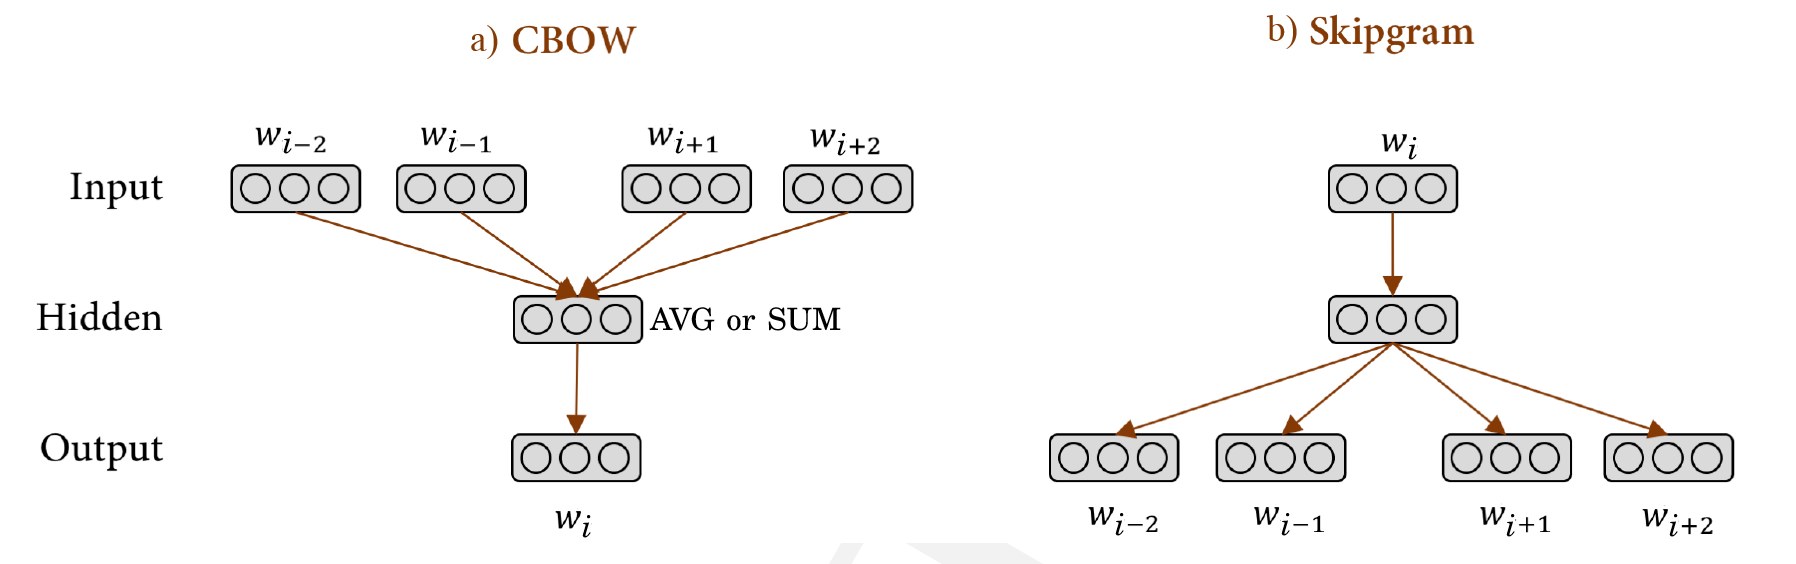
\includegraphics[width=\linewidth]{Pictures/Pilehvar_20_w2v.png}
    \caption{Adapted and modified from \citet{embedding2020pilehvar}: Visualization of the two prediction tasks present in the Word2Vec framework with a window size of 2. \newline 
    a) CBOW: $w_i$ constitutes the target word which shall be predicted using the two preceding and subsequent words. \newline
    b) Skipgram: $w_i$ constitutes the input (middle word) which shall be used to predict the two preceding and subsequent words.}
    \label{fig:w2v}
\end{figure}

Figure \ref{fig:w2v} b) visualizes the second architecture, the skipgram approach. Here $w_i$ serves as the input to the model, is fed to the projection layer and a log-linear classifier tries to predict the words in the context \citep{mikolov2013efficient}, in this case $w_{i-2}, w_{i-1},w_{i+1},w_{i+2}$. Therefore one instance for the training process is the tuple of the middle word $w_i$ and either one of its context words as a positive example or a word that does not appear in its context as a negative example. 

Since such tuples could be created for each combination of the vocabulary and this would result in innumerous cases, the process called negative sampling chooses a limited number of combinations of the middle word and words that did not appear in its context \citep{karimi2021sampling}.
Additionally since the relatedness of words declines once you move further away from a certain word, combinations of the middle word and words in its context, but relatively far away, are sampled less frequently \citep{mikolov2013efficient}.

For both architectures the log-linear classifier then has to distinguish the positive cases in which the samples are made up of words that belong to the same context and the negative samples \citep{jurafsky2021}.

Once the training process for the prediction task is finished, it is no longer relevant since the word embeddings are obtained by extracting the weight matrix of the projection layer \citep{mikolov2013efficient}.

As shown by \citet{mikolov2013efficient} these techniques result in word embeddings that provide valuable information on the syntactic and semantic relatedness of words when trained on very huge datasets.

The fact that for training the word embeddings the running text itself provides the input and correct output like a supervised task is called self-supervision and provides, as \citet{jurafsky2021} put it, a 'revolutionary intuition' for effective word embedding training.






\subsection{FastText}
\label{word_fasttext}
One shortcoming of the Word2Vec framework is that it only assigns distinct embeddings to words. In cases of corpora with many rare words, this may result in missing embeddings for words that have not been in the training corpus \citep{bojanowski2017enriching}.

To bypass this limitation by providing word embeddings for a high percentage of before unseen words, the concept of implementing the prediction tasks of chapter \ref{word_w2v} additionally at the level of constituent character n-grams for each word is realized. This technique was developed as an extension of the Word2Vec framework, called FastText \citep{bojanowski2017enriching}. 

Especially since many before unseen words are morphological variations of words that exist in the vocabulary \citep{embedding2020pilehvar}, the enabling of learning these different morphological forms of words without necessarily encountering each form in its completeness in the corpus provides valuable data \citep{jain2016fasttext}. 

So the representations of words are learned by summing up the embeddings learnt for the constituent n-grams and the word itself \citep{rehurek2022fasttext}. 

If one considers the word 'fastext' and character n-grams of length 3, the resulting sequence on which sub-word character ngram embeddings are learnt is made up of:

\begin{quote}
    \label{char-n-grams}
    \centering
    $<$fa,  fas,    ast,    stt,    tte,    tex,    ext,    xt$>$
\end{quote}

'$<$' and '$>$' are considered special boundary symbols to delimit the word boundaies \citep{jurafsky2021}.

Once a before unseen word is encountered, the FastText framework creates its word embedding by averaging its constituent sub-word embeddings. Thereby providing a reasonable alternative to assigning 0-vectors or random numbers as word embeddings for these words with the drawback that words may incorporate the same constituent sub-word n-grams without being semantically related \citep{embedding2020pilehvar}.


\subsection{GloVe}
\label{word_glove}
The Word2Vec and FastText framework provide word embeddings that utilize local context window methods, the prediction tasks discussed in chapter \ref{word_w2v}, to enable them to perform considerably well on analogy tasks regarding their semantic relatedness. Though statistical information like the global co-occurrence counts are mostly disregarded by these frameworks and thereby they miss potential leverage for the quality of the word embeddings as they do not take advantage of the vast amount of repetition in the data \citep{pennington2014glove}.

In contrast, the GloVe framework directly utilizes the global corpus statistics which gave rise to its name \citep{jurafsky2021}.

Another key difference to the two before mentioned frameworks is that GloVe uses no neural network in its model, but introduces an optimization problem to construct the word embeddings \citep{embedding2020pilehvar}.
While a neural network could have been deployed in the construction of this framework, \citet{pennington2014glove} have made a point against this, since it would obfuscate the linear structure of the word embeddings they were trying to capture.

The key idea behind the GloVe framework is to use co-occurrence probabilities of words and their ratios \citep{jurafsky2021} to build an objective function which is optimized by stochastic gradient descent \citep{embedding2020pilehvar}.
This objective function is built on the hypothesis that semantic relationships can be effictively captured by computing the ratio of co-occurrence probabilities for three words $w_i,w_j,w_k$. Consider $P_{i,k}$ as the probability of the word $w_k$ occurring in the context of word $w_i$.

\begin{equation}
    \label{eq:ratio}
    P_{i,k}/P_{j,k}
\end{equation}

Then the ratio (\ref{eq:ratio}) is expected to be large if $w_i$ and $w_k$ have a semantic relatedness, co-occur often, while $w_j$ and $w_k$ have no semantic relatedness, seldom co-occur. It is expected to be small in the vice-versa case. If neither or both, $w_i$ and $w_j$, have a semantic relatedness to $w_k$, the before mentioned ratio is expected to be near 1. All these hypotheses have been exemplified in \citet{pennington2014glove}.

As the before mentioned ratio is based on three different words $w_i,w_j,w_k$ and can be the source of information on their semantic relatedness, the objective function that is optimized in the GloVe framework has been modified as to capture the information inherent in such ratios in the word embeddings of the respective words \citep{pennington2014glove}.

\citet{pennington2014glove} have shown in their result chapter that the GloVe framework may outperform Word2Vec on word analogy tasks and provide the word embeddings in a shorter time span under similar conditions.


% Begin Practical Part 

\section{The Georgetown University Multilayer Corpus} % and possible other datasets
The Georgetown University Multilayer Corpus (GUM) is an open source collection of texts of multiple types which get annotated extensively \citep{ud2022opencom}. At the Georgetown University students collect and expand the corpus as a part of their curriculum by adding layers of analysis to a text chosen from openly available sources \citep{Zeldes2017}.

The POS-tags are manually annotated using the Stanford Typed Dependencies \citep{de2008stanford} and are converted to the Universal Dependencies tagset using the DepEdit tool \citep{ud2022opencom}. Afterwards the tags are corrected manually using the Universal Dependencies guidelines, to ensure the quality of the annotations.

The text types used in the data are meant to represent a variety of communicative purposes and stem from openly available sources to prevent restrictive licenses from interfering with the process of annotating and publishing.
Sources include Wikinews, Wikipedia and reddit, while the text types are divided in categories in such as interviews, news articles, biographies and fiction \citep{Zeldes2017}.

The fact of being open source helps making the analysis reproducible. Being compiled by the Georgetown University ensures that the data follows institutional guidelines and quality standards, while the corpus size of roughly 7 thousand sentences allows for reasonable computability speeds on machines with an average computing capability. Therefore the choice of data for this thesis has been the GUM dataset.
\label{gum}


\section{Implementation}

\subsection{CoNLL-U format and data extraction}
\label{conllu_imp}
First of, it needs to be said that all programming related notions are done using the programming language Python.

The data of the Georgetown University Multilayer Corpus is openly avaible on the Universal Dependencies website where it is provided in the CoNLL-U format. This format encodes the data in plain text form using the LF character as line breaks and incorporates lines containing information on words, comment lines and blank lines marking the boundary of a sentence \citep{ud2022opencom}.

Sentences are made up by at least a single word line which possesses 10 fields with information on the syntactic nature and dependencies of its words.

As this thesis explores the predictive power of linguistic features for POS-tagging in settings where just the plain text is being provided, the fields that are extracted are simply the 'form' which is present in the sentence and the respective 'UPOS' which is one of the 17 tags in the Universal Dependencies tagset, presented in chapter \ref{pos_tagsets}. The latter will be considered the gold standard for the task in general.

While some of the remaining 8 fields of the words may hold valuable information for the prediction of tags, these were not extracted since they are not accessible once a corpus without annotations is presented to the POS-tagging model.

\citet{Zeldes2017} provided the data already split in a train, development and test set while ensuring that the discussed text types in chapter \ref{gum} are balanced equally in them.

So after importing the data from the CoNLL-U format to Python, a list of sentences which themselves are lists of tuples with word form and the respective tag is provided for each of the sets. 
The training set contains roughly one hundred thousand tagged words while the development and test set compromise about 16 thousand respectively.

\subsection{Simple feature extraction and encoding}
\label{feat_imp}
Once the data is retrieved in Python in form of a list of sentences which themselves are lists of tuples (the word and their respective tag), the features for the POS-tagger have to be extracted.

As neural networks provide the framework for our model, all features have to be encoded in a numeric fashion.

The features used in this thesis are grouped into classes to limit the combinations for which to run the evaluations of the models since the computational cost of training thousands of neural networks to cover all possible combinations of single features was not feasible.

First of is the group of features that concerns itself with the class of characters a word encompasses. Therefore five features have been encoded in a binary fashion (either 0 or 1) to check for different characteristics of the associated characters of a word. It is checked whether a word is made up of purely alphabetic characters, purely numeric characters, purely alphanumeric characters, whether it contains at least one numeric character and whether it contains a hyphen. In positive cases these features are encoded with the value 1 and else with 0. From now on this class of features will be referred to as the character related features.

Secondly, a feature group of four deals with the case of characters in a word. They check whether a word starts with a capital letter, it has a capital letter after the first character, is completely upper case or completely lower case. This group will be referred to as the case related features.

Thirdly a group of two features checks whether a word appears at the beginning or end of a sentence and will therefore be called the sentence position related features.

The final group of features concerns itself with affixes of words, prefixes and suffixes. To get information on the prefixes that may be encompassed in a word, a list of the most common English prefixes according to the Cambridge Dictionary \citep{cambridge2022prefix} was used to search for words with these prefixes in the training data. 
For prefixes found in the training data the most common tag for words with the respective prefix has been set as the default tag which will be encoded for all words with such a prefix.
Similarly, suffixes are searched for by using a stemmer provided by the NLTK package. Again, for suffixes that have been found in the training data the most common tag for each respective suffix will be encoded for words that encompass it.
For both, prefixes and suffixes, it is checked how many different tags, that were most common to words with a certain affix, were encountered. Afterwards a one-hot-encoding is created with length respective to the different tags, found as mentioned before, in which the position of the tag, which was the most common tag for a certain affix, is encoded with a 1 if this affix is found in a word. Thereby the two features for prefixes and suffixes result in one-hot-encodings with varying length indicating which tag was most common to a known affix in the training data. This group will be referred to as the affix related feature group.


\subsection{LSTM Neural Network}
\label{lstm_imp}
The task of POS-tagging utilizes intrinsic and extrinsic features of words in a sentence as its input values as described in chapter \ref{pos_features}. Sentences can be considered as sequential data, a sequence of words.

To ensure the preservation of the structural properties of sequential data Recurrent Neural Networks are appropriate, while the task of retaining information of previous predictions and avoiding vanishing gradients in the training process of neural network makes LSTM Neural Networks the choice for the model architecture for the POS-tagging task.

In Python LSTM Neural Networks can be implemented using the Keras package. Therefore a sequential model ($keras.models.Sequential$) was defined. As the sole hidden layer in this model a LSTM layer ($keras.layers.LSTM$) was appended with a varying number of units ($unit\_count$) which are specified by other modules in this thesis. Afterwards the output layer is added which contains as many units as the tagset contains different tags. So in case of using the Universal Dependencies tagset, it has 17 units on which the $softmax$ function is applied. The compilation of this model was done with the optimizer called $adam$ and the Cross-Entropy loss function was implemented.

The number of input units for this model was not specified to ensure the model's setup to be adaptable to the varying number of features that are used in the different evaluation processes.

To enable feeding the whole set of training data for fitting the model, the sentences need to have a fixed length. Therefore the length of the longest sentence in the data is used as the length for all the other sentences which are padded with zero vectors to fill the difference in their length.

All models mentioned in this thesis use this LSTM Neural Network's setup for the task of POS-tagging and are therefore often referred to simply as the POS-tagging models. If the sole input of such a model is the implementation of a certain word embedding framework, the LSTM Neural Network given the POS-tagging task is often referenced by the name of the word embedding framework plus 'model'.


\subsection{Encoding word identity with word embeddings}
\subsubsection{Word2vec}
\label{word2vec_imp}
To encode the word identity, all word embedding frameworks presented in chapter \ref{we} were utilized and in the case of Word2Vec and FastText self-trained on the training data with the Gensim package.

For the Word2Vec framework 216 different word embeddings have been trained using all possible combinations of values for the hyperparameters which will be discussed in the following paragraphs and the two architectures of Word2Vec.

As the $gensim.models.Word2Vec$ function comes with numerous hyperparameters for regulating the training process of the Word2Vec word embeddings, all hyperparameters not mentioned here were given their default value. 

First of is the hyperparameter, called $min\_count$, which filters all words that have occurred at least as often as the value it is set to. Words that have occurred fewer times in the used corpus are disregarded for in the training procedure. Values used in the thesis are 1, 2, 3 and 5 which are relatively low values considering the default value to be 5, but given the limited corpus size this choice was deemed reasonable.

Next of is the window size ($window$) which regulates the prediction task as explained in chapter \ref{word_w2v}. In this thesis the values 2, 3 and 5 were employed, though these are again rather on the low side of values given the default value to be 5. This choice was made on the basis that the syntactic relatedness of words declines sharply with the distance between them which is of main concern to the task of POS-tagging.

The third hyperparameter for which different instantiations were utilized is the vector size ($vector\_size$) of the resulting word embeddings. As the default for this parameter is 100, the values used in this thesis are 50, 100 and 200 to test for the quality of word embeddings with dimensionalities of the default value, a lower value and a considerably higher value.

Afterwards the hyperparameter called $alpha$ which is the learning rate of the training algorithm was tuned with the values of 0.015, 0.03 and 0.045. These values were chosen as to reasonably cover the different learning rates relative to the default value of 0.025.

All the before mentioned values of hyperparameters were used in combination with the two architectures, CBOW and SG, to create the 216 different word embeddings with the Word2Vec framework.

The hyperparameter of the minimal learning rate ($min\_alpha$), which constitutes the bottom line for the linearly decreasing learning rate ($alpha$) as training progresses, was set to the quotient of $alpha$ and the default value of the training epochs (5). This results for all applied learning rates in a much higher value than its default value 0.0001. This was done since the amount of data used for training the word embeddings (the GUM training data) is much smaller than the size of data \citet{mikolov2013efficient} used in their paper.

For all created Word2Vec word embeddings two LSTM Neural Networks, see chapter \ref{lstm_imp}, for the POS-tagging task are created. The first has 75 units in the hidden LSTM layer and the second one has 125. The accuracy of these models should be the basis on which to decide the quality of the different Word2Vec word embeddings when these are the only features provided for the POS-tagging model.



\subsubsection{FastText}
\label{fasttext_imp}
As mentioned in chapter \ref{word_fasttext}, the FastText framework was developed as an extension to Word2Vec. Therefore it was deemed reasonable to build different FastText models with the hyperparameters of the best performing Word2Vec word embeddings and thereby limit the combinations of parameters for which FastText word embeddings are created.

As mentioned in the last paragraph of chapter \ref{word2vec_imp}, each Word2Vec model has been evaluated with two different LSTM Neural Networks which differ only in their number of units in the hidden layer. The accuracy of these models decides which word embeddings have performed best on the POS-tagging task.

In this thesis the five best performing Word2Vec word embeddings will provide most of the hyperparameters for the FastText models and are combined with two additional hyperparameters which are inherent to the FastText framework. FastText models incorporate sub-word information by considering character ngrams. This is done by defining the range of character ngrams that should be embedded using the hyperparameters, minimum ($min\_n$) and maximum ($max\_n$) character sequence length. While the $gensim.models.Fasttext$ function incorporates the minimum and maximum as separate parameters, they were treated as a tuple in this thesis. The ranges used for training the FastText word embeddings were (2, 5) and (3, 6).

This resulted in 10 different FastText word embeddings, 5 different sets of hyperparameters of the best performing Word2Vec models times the 2 different characters ranges for character ngrams. These were evaluated in the same way as described in chapter \ref{word2vec_imp} and use the same $unit\_count$(s) as the Word2Vec models on which they are based.

\subsubsection{GloVe}
\label{glove_imp}
As there exists no module to implement the GloVe framework to train word embeddings on specific data in Python, pre-trained word embeddings from \citet{pennington2014glove} were utilized. They were originally trained on a corpus of 6 billion words compiled from Wikipedia and the English Gigaword archive.

The pre-trained word embeddings come with a vector size of 50, 100, 200 and 300. To maintain a valid comparability between the different word embedding frameworks only the 50, 100 and 200 dimensional ones were considered. As for the other two frameworks, these three different GloVe word embeddings were tested on their performance for the POS-tagging task on the training data by the accuracy of a LSTM Neural Network with the word embeddings as their sole input with the two different numbers of units in the hidden layer (75, 125).


\subsection{Workflow of the evaluation process}
\label{workflow_imp}
All the previously described implementations are combined and controllable via a main script.

The overall workflow of this script includes 8 major steps. 


First of is the creation of Word2Vec word embeddings with the different hyperparameters and archictectures which are described in chapter \ref{word2vec_imp}. These are parameters of the main script (see $we\_min\_count$, $we\_window\_size$, $we\_vector\_size$, $we\_alpha$, $we\_implementation$ in table \ref{tab:parameters}) and are configurable in the console.

Secondly the created Word2Vec embedding(s) that are specified by the parameters of the main script is evaluated by computing the accuracy the LSTM Neural Network has achieved on the POS-tagging task with the word embedding as its sole input. This neural network contains the number of units in the LSTM layer specified by a parameter of the main script (see $unit\_count$ in table \ref{tab:parameters}) which is configurable. Each evaluated Word2Vec model is documented with its accuracy in a CSV file.

The third step searches for the five best performing Word2Vec models evaluated as described in step two, even if they were evaluated in another session, supposing there are already as much as 5 evaluated in the respective CSV file. The selected Word2Vec models provide the hyperparameters for the FastText word embeddings as described in chapter \ref{fasttext_imp} and the range for the character ngrams is supplied by parameters of the main script (see $ft\_char\_range\_min$, $ft\_char\_range\_max$ in table \ref{tab:parameters}) and is thereby again directly configurable in the console.

Next comes the evaluation of the created FastText word embeddings which happens similarly to step two for the Word2Vec models and is executed for all FastText word embeddings that are specified by the creation process of step 3 with the same number of units as was specified for step 2 ($unit\_count$). These evaluations have a respective CSV file to document the performance of the FastText models.

As the fifth step of the main script workflow, the GloVe word embedding(s) is evaluated by selecting the pre-trained word embedding with the vector size according to a parameter of the main script (see $glove\_dimensions$ in table \ref{tab:parameters}) and, as for the other frameworks, a LSTM Neural Network with the before specified number of units in its hidden layer ($unit\_count$) is evaluated by computing the accuracy on the POS-tagging task and documented in a CSV file.

The sixth step searches for all word embedding frameworks the best performing model, which was at some point evaluated by step 2, 4 and 5, in the respective CSV file. This will not necessarily be the word embeddings specified by the parameters of the main script that were chosen for this particular execution of the script. These 3 models will provide the word embeddings and the number of units in the hidden layer of the POS-tagging model for the final evaluations in step 7.

Afterwards, in the seventh step the three best performing models of each word embedding framework with their respective $unit\_count$ are evaluated thoroughly in combination with the feature groups that are either included or excluded through the parameters of the script (see $eval\_char\_related$, $eval\_case\_related$, $eval\_sent\_position$, $eval\_affixes$ in table \ref{tab:parameters}) and are described in chapter \ref{feat_imp}. Additionally it can be regulated whether the word embeddings are placed at the beginning or the end of the encoded features for a word by the parameter $eval\_we\_end$.
For the resulting POS-tagging models dictionaries are created and saved as JSON files which include several evaluation metrics. For each tag in the tagset the precision, recall and F1-score is computed individually. Overarching the individual tags the macro precision, macro recall, macro F1-score, weighted precision, weighted recall, weighted F1-score and the general accuracy are computed and added to the dictionary.

Finally, in step 8, for all thoroughly evaluated models the macro precision, macro recall, macro F1-score, weighted precision, weighted recall, weighted F1-score and accuracy are printed to the console. This is done for all models that have been evaluated at any point in time in step 7 and therefore have a respective dictionary with their evaluation.

\newcommand*{\thead}[1]{\multicolumn{1}{c}{\bfseries #1}}

\begin{table}[]
\centering
\label{tab_parameter}
\begin{tabular}{|l|l|l|}
\thead{Parameter name} & \thead{Description} & \thead{Covered} \\
\hline
we\_min\_count       & Minimal word count for W2V/FT creation       & {[}1, 2, 3, 5{]}         \\
we\_window\_size     & Window size for W2V/FT creation              & {[}2, 3, 5{]}            \\
we\_vector\_size     & Vector sizes  for W2V/FT creation            & {[}50, 100, 200{]}       \\
we\_alpha            & Alpha (learning rate) for W2V/FT creation    & {[}0.015, 0.03, 0.045{]} \\
we\_implementation   & Architecture for W2V/FT creation             & {[}'cbow', 'sg'{]}       \\ \hline
ft\_char\_range\_min & Minimum character range for FT creation      & {[}(2, 5), (3, 6){]}     \\
ft\_char\_range\_max & Maximum character range for FT creation      & {[}(2, 5), (3, 6){]}     \\ \hline
glove\_dimensions    & Vector size for GloVe embedding selection       & {[}50, 100, 200{]}       \\ \hline
unit\_count          & Unit count for the LSTM layer in POS-tagger        & {[}75, 125{]}            \\ \hline
eval\_char\_related  & Binary: Include character related features    & {[}0, 1{]}               \\
eval\_case\_related  & Binary: Include case related features         & {[}0, 1{]}               \\
eval\_sent\_position & Binary: Include sentence position r. features & {[}0, 1{]}               \\
eval\_affixes        & Binary: Include affix related features       & {[}0, 1{]}               \\
eval\_we\_end        & Binary: Place word embedding at the end            & {[}0, 1{]}               \\ \hline
\end{tabular}
\caption{Parameters to regulate the behaviour of the main script. The columns include the parameter name, a description of its function and values used in the complete evaluation.}
\label{tab:parameters}
\end{table}

To reproduce all the created word embeddings, their respectively evaluated POS-tagging models and the thorough evaluations of the best word embeddings models per framework with all the different combinations of feature groups, it is recommended to change the code of the main script by commenting out the specific parameters given to the main script by the console arguments and instead use the list of choices for those parameters (see column 3 in table \ref{tab_parameter}) that are present in the script but are commented out. 



\section{Results}

\subsection{Word embeddings}
\label{res_we}
As explained in chapter \ref{workflow_imp}, a first evaluation on the basis of the accuracy on the POS-tagging task was done to decide which word embeddings in combination with a certain number of units in the hidden layer of the LSTM Neural Network model ($unit\_count$) perform the best for each of the three covered frameworks.

Each framework was individually evaluated to decide the most favorable hyperparameters, architecture (in case of Word2Vec and FastText) and the best performing amount of units in the hidden layer (in case of all frameworks). The only hyperparameter to differentiate for between the pre-trained GloVe word embeddings is their vector size.

\begin{table}[]
\centering
\begin{tabular}{lllllll}
\thead{min\_count} & \thead{window} & \thead{vector\_size} & \thead{alpha} & \thead{architecture} & \thead{unit\_count} & \thead{accuracy}  \\
\hline
2 & 3 & 200 & 0.045 & SG & 125 & 0.696 \\
5 & 5 & 200 & 0.045 & SG & 125 & 0.692 \\
2 & 2 & 200 & 0.045 & SG & 125 & 0.690 \\
3 & 2 & 200 & 0.045 & SG & 125 & 0.688 \\
3 & 5 & 200 & 0.045 & SG & 75 & 0.687
\end{tabular}
\caption{Hyperparameters, architecture and number of units in the hidden layer of the model of the five best performing Word2Vec models sorted by accuracy}
\label{tab:w2v}
\end{table}

In table \ref{tab:w2v} the five best performing Word2Vec models are listed by their hyperparameters, architecture and the number of units used in the LSTM layer of the POS-tagging model. 
One can surmise from this table that a high vector size, a high learning rate, the SG architecture and the higher amount of units in the hidden layer make a POS-tagging model perform better on the GUM dataset. It could be speculated that higher vector sizes and numbers for the $unit\_count$ parameter enable the model to represent more complex attributes that are valuable to the POS-tagging task. The fact that the highest of the three covered learning rates performed best could indicate that with the limited amount of data available the pace of learning needs to be relatively high to enabling the training process to encode valuable structural properties.

Given the information in table \ref{tab:w2v}, the final evaluation of the utility of linguistic features used a Word2Vec word embedding with the hyperparameters and architecture of the uppermost model in the table and the respective $unit\_count$ in the POS-tagging model. This will be the foundation of the final analysis given that one uses the Word2Vec framework for word embeddings.

The five models present in table \ref{tab:w2v} specify the hyperparameters $min\_count$, $window$, $vector\_size$, $alpha$, the architecture and number of units ($unit\_count$) for the creation of FastText word embeddings and the respective LSTM Neural Networks that are build with them as their sole input.

\begin{table}[]
\centering
\begin{tabular}{llll}
\thead{Word2Vec model basis} & \thead{min\_n} & \thead{max\_n} & \thead{accuracy}  \\
\hline
w2v\_2\_3\_200\_045\_sg\_125 & 2 & 5 & 0.698 \\
w2v\_2\_2\_200\_045\_sg\_125 & 2 & 5 & 0.692 \\
w2v\_3\_2\_200\_045\_sg\_125 & 2 & 5 & 0.692 \\
w2v\_3\_5\_200\_045\_sg\_75 & 2 & 5 & 0.669 \\
w2v\_2\_2\_200\_045\_sg\_125 & 3 & 6 & 0.664
\end{tabular}
\caption{The first column displays the Word2Vec model basis which supplies the $min\_count$, $window$, $vector\_size$, $alpha$, architecture parameters for the FastText word embeddings and the number of units in the hidden layer ($unit\_count$) for the resulting model. The second and third column are the hyperparameters characteristic to FastText word embeddings and the last column is the accuracy of the resulting model.}
\label{tab:ft}
\end{table}

In table \ref{tab:ft} the five best performing FastText models are presented which incorporate subword information by providing embeddings for character ngrams in the ranges of (2,5) and (3,6). These models yield no considerably better results regarding the accuracy in the POS-tagging task on the GUM dataset than the Word2Vec models.

The first column in table \ref{tab:ft} describes the Word2Vec model basis. It follows the notational approach that was used throughout this thesis. 
Word embeddings and the evaluations for their models are saved and referenced by a naming convention that uses underscores to separate their integral parts.
First comes an abbreviation for the word embedding framework, afterwards, separated by underscores, parameters that were covered in this thesis and belong to this respective framework and finally, if the name refers to the evaluation of the respective POS-tagging model, the number of units in its hidden layer is written at the end. 

For example w2v\_2\_3\_200\_045\_sg refers to the Word2Vec word embedding with $min\_count$ 2, $window$ 3, $vector\_size$ 200, $alpha$ 0.045 and the SG architecture.

In w2v\_2\_3\_200\_045\_sg\_125 the appended '\_125' at the end indicates that it refers to the evaluation of the LSTM Neural Network with 125 units in the hidden layer and the before mentioned word embeddings as its sole input.

For the final analysis the FastText model specified by the top row in table \ref{tab:ft} will serve as the base model regarding the FastText framework.

\begin{table}[]
\centering
\begin{tabular}{lllllll}
\thead{vector\_size} & \thead{unit\_count} & \thead{accuracy}  \\
\hline
200 & 125 & 0.811 \\
100 & 125 & 0.804 \\
200 & 75 & 0.797 \\
100 & 75 & 0.791 \\
50 & 75 & 0.664 \\
50 & 125 & 0.655
\end{tabular}
\caption{Vector size of the pre-trained GloVe embeddings and the number of units in the hidden layer for the resulting model ($unit\_count$) sorted by the third column, the accuracy on the POS-tagging task.}
\label{tab:glove}
\end{table}

As for the GloVe framework, all six combinations of vector sizes ([50, 100, 200]) and numbers of units for the hidden layer of the POS-tagging model ([75, 125]) are evaluated considering their accuracy and depicted in table \ref{tab:glove}. The evaluation of linguistic features will use a GloVe model with vector size 200 for the word embedding and a $unit\_count$ of 125 for the respective POS-tagging model.

\subsection{Utility of linguistic features}
\label{res_feature}
For each of the three different word embedding frameworks, one model, presented as the best performing for one framework in the previous chapter, is utilized to analyse the utility of the different linguistic features. This is done by expanding the input the model receives by the different feature groups of chapter \ref{feat_imp}.

\begin{figure}
    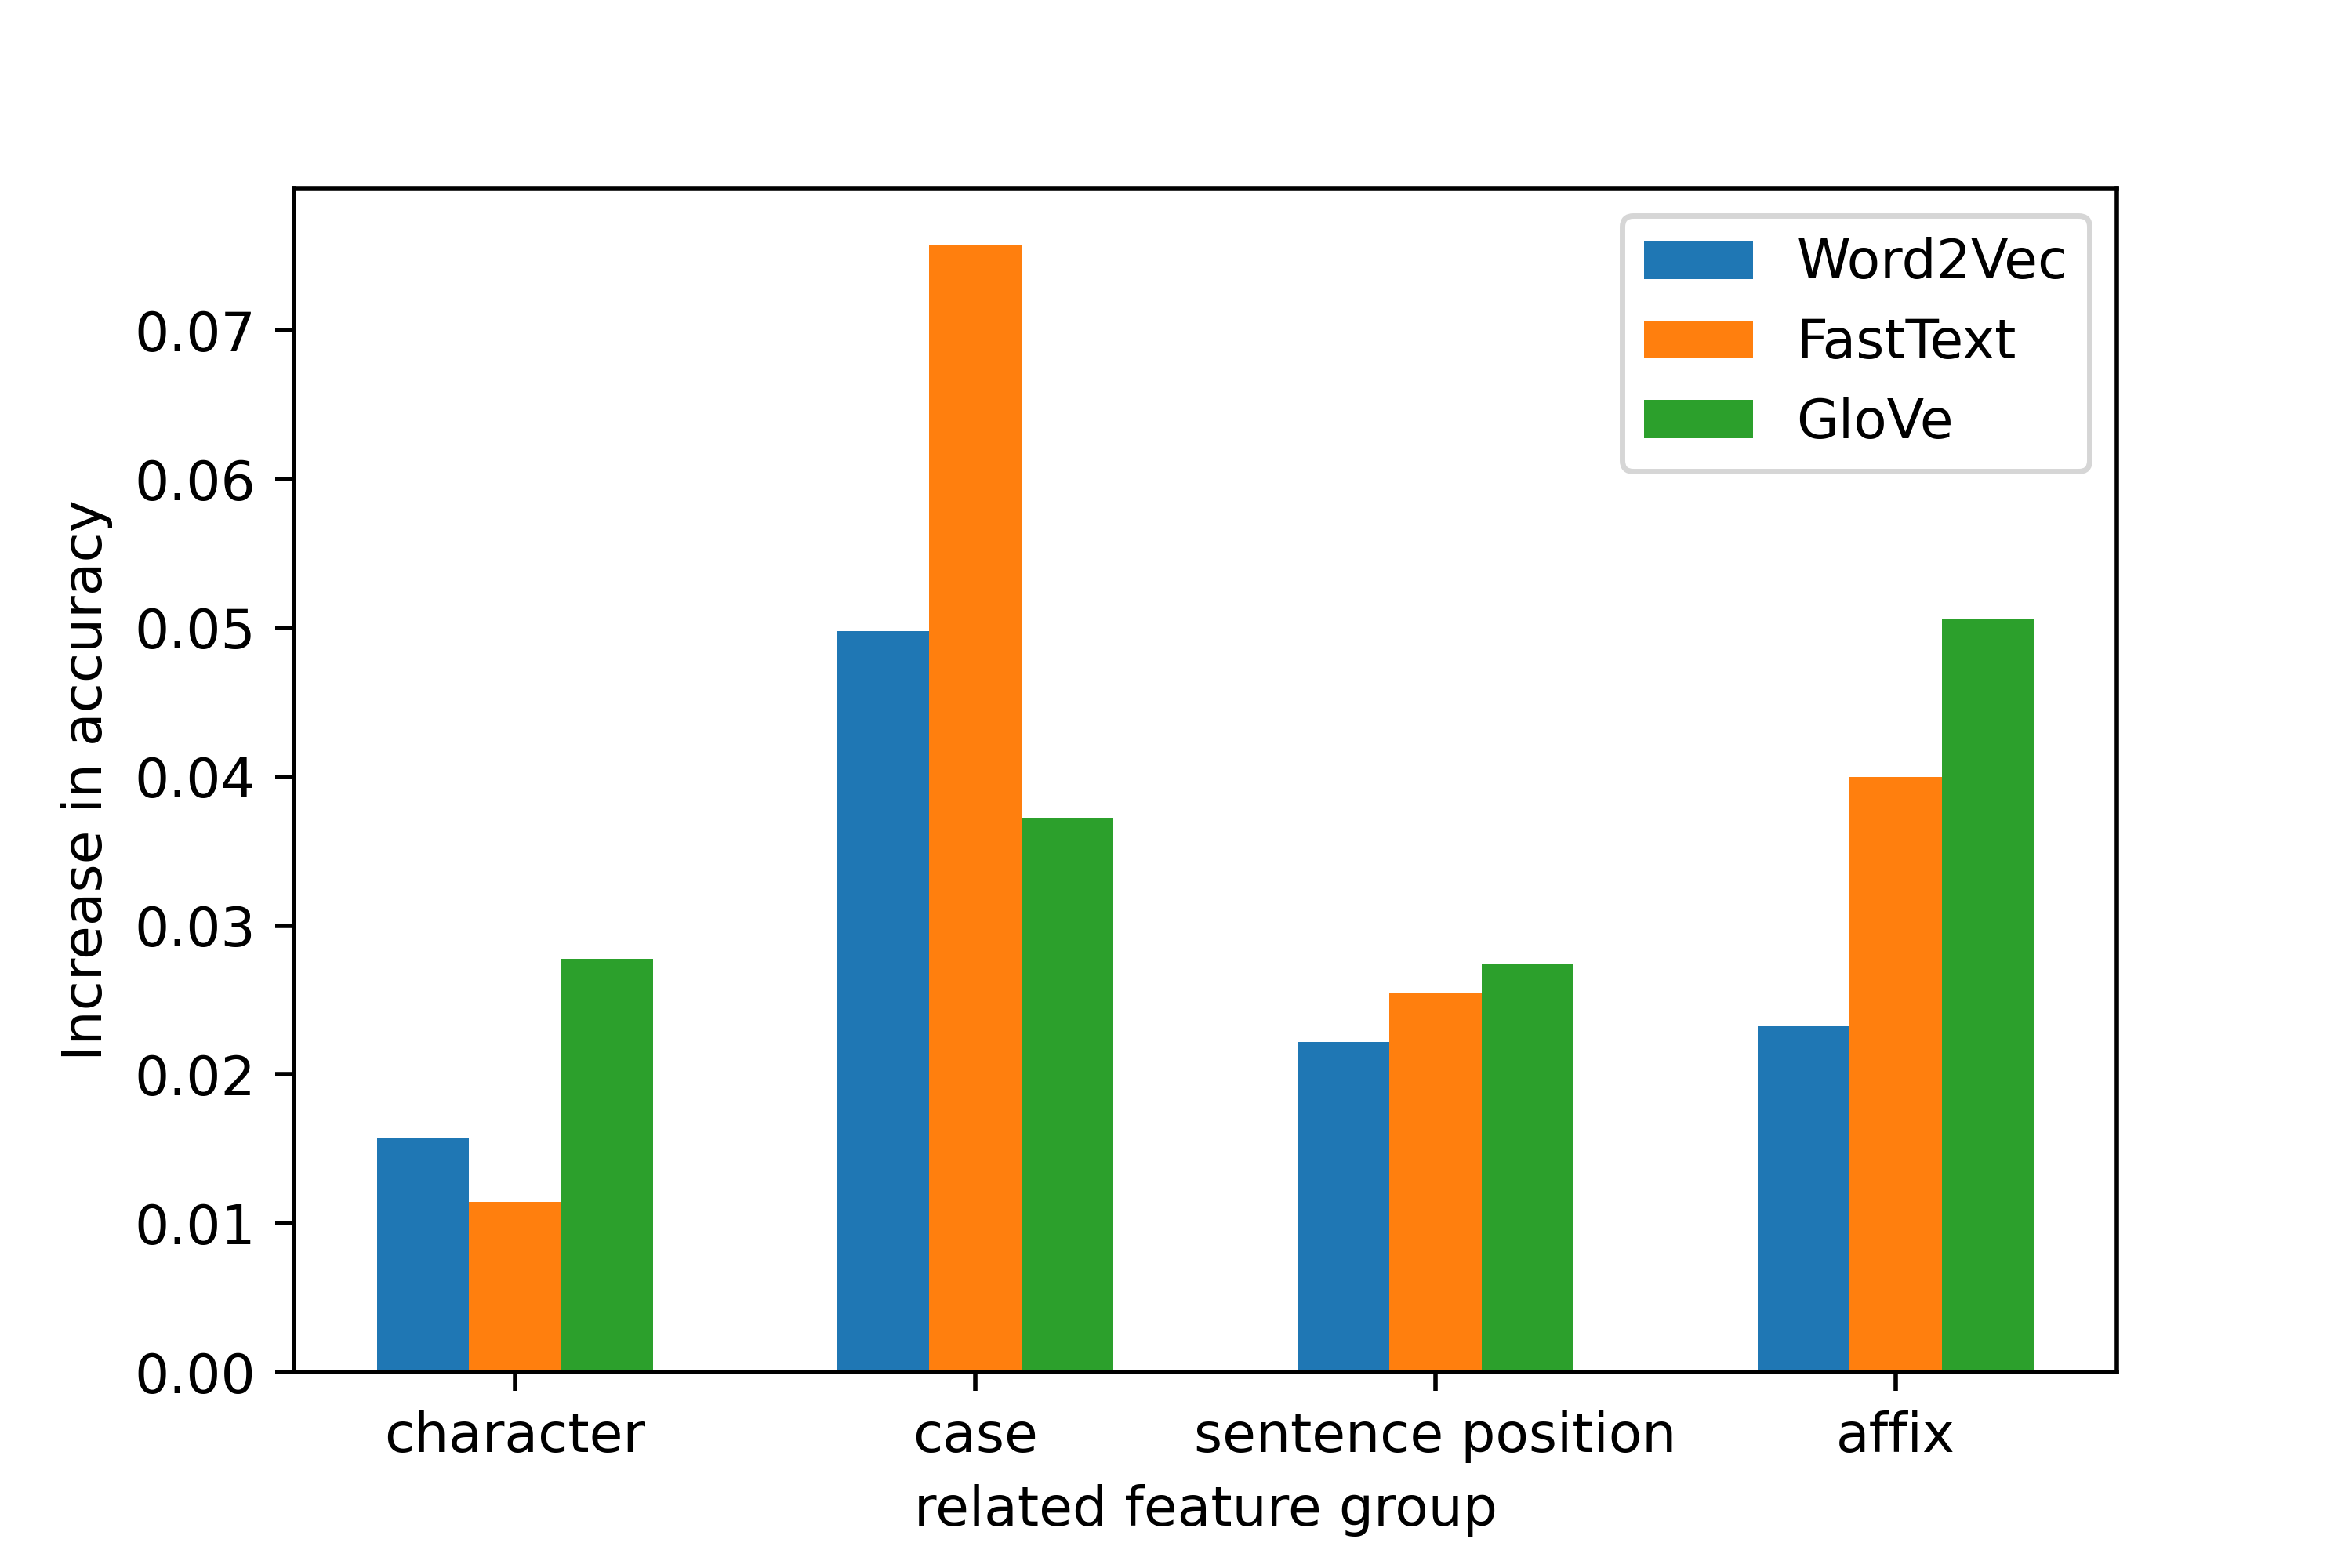
\includegraphics[width=\linewidth]{Pictures/accuracy_gain.png}
    \caption{Bar plot of the increase in accuracy of the POS-tagging model once one of the four feature groups is incorporated in the model in comparison to the model with the respective word embedding as its sole input.}
    \label{fig:acc}
\end{figure}


In figure \ref{fig:acc}, the gain in accuracy is depicted once a certain feature group is incorporated compared to the model with the word embedding as its sole input. It can be seen that the groups of character related and affix related features provide the biggest gain in accuracy for the POS-tagging models while the group of character related features is the least informative for the Word2Vec and FastText model.

\begin{table}[]
\centering
\begin{tabular}{|l|l|l|l|l|}
\thead{Framework} & \thead{related features} & \thead{accuracy} & \thead{weighted F1} & \thead{macro F1} \\
\hline
Word2Vec & character         & 0.0191 & 0.0235 & 0.0407 \\
Word2Vec & case              & 0.0528 & 0.0494 & 0.0480 \\
Word2Vec & sentence position & 0.0268 & 0.0340 & 0.0435 \\
Word2Vec & affix             & 0.0500 & 0.0614 & 0.0495 \\ \hline
FastText & character         & 0.0102 & 0.0143 & 0.0223 \\
FastText & case              & 0.0646 & 0.0614 & 0.0611 \\
FastText & sentence position & 0.0294 & 0.0343 & 0.0435 \\
FastText & affix             & 0.0368 & 0.0468 & 0.0402 \\ \hline
GloVe    & character         & 0.0079 & 0.0080 & 0.0094 \\
GloVe    & case              & 0.0219 & 0.0228 & 0.0255 \\
GloVe    & sentence position & 0.0157 & 0.0176 & 0.0242 \\
GloVe    & affix             & 0.0332 & 0.0360 & 0.0270 \\ \hline
\end{tabular}
\caption{Average increase in the metrics accuracy, weighted F1-score and macro F1-score once a feature group is added compared to each model that does not incorporate that feature group.}
\label{tab:feat_group}
\end{table}


Table \ref{tab:feat_group} shows the change in model performance on the POS-tagging task once a certain feature group is included in the LSTM Neural Network compared to the model without the information of this feature group. 

The values are obtained by averaging the distance in the metrics between models that incorporate that feature group and ones that do not while being exactly similar in all other aspects. 
For the POS-tagging models with the self-trained word embeddings, utilizing the group of case related features results in biggest increase in all but one of the depicted evaluation metrics. 

For models with the GloVe word embedding, the incorporation of the group of affix related features produces the biggest increase in the evaluation metrics. This may have been due to a incapability of the GloVe framework to capture meaningful sub-word level information while being high quality word embeddings in general (since the embedddings were pre-trained on huge amounts of data).

Word2Vec models have a bigger increase in the metrics if the affix feature group is utilized compared to the FastText models which could indicate that the FastText framework was able to capture meaningful sub-word level information regarding affixes on itself.

The performance of the POS-tagging models on the level of individual tags varies strongly, but the tendency that tags that occur seldom in general are mostly ignored can be shown by the fact that for the tag 'X' which has occurred only 252 times in the training data all POS-tagging models have a F1-score of 0 for this tag.

No meaningful change in model performance was perceived by changing the word embedding position from the beginning of the input space to its end.

Overall, the combinations of feature groups, the word embedding position and the three frameworks for word embeddings resulted in 93 POS-tagging models that were evaluated with the before mentioned metrics. The best perfoming POS-tagging model was a LSTM Neural Network with 125 units in its hidden layer, the GloVe word embedding with vector size 200 and all feature groups as its input. It has achieved an accuracy of 0.882 and a weighted F1-score of 0.877.

As a baseline for putting the evaluated models in perspective, a tagger was build that assigns the most common tag for a word in the training data to each respective word that was encountered and the the most common tag in general ('NOUN') to before unseen words. This baseline tagger has achieved an accuracy of 0.828 on the POS-tagging task on the GUM data. 26 of the 93 thoroughly investigated LSTM Neural Networks have performed on this task with a higher accuracy. 24 of them incorporated the pretrained GloVe word embeddings while two of them used the self-trained Word2Vec word embeddings.



\section{Discussion and Conclusion}
As mentioned at the end of the previous chapter, only about a third of the POS-tagging models beat the baseline tagger with regards to the accuracy on the GUM data. This begs the question what limitations of the self-build models may have caused such an outcome.

Firstly, the self-traind  word embeddings need to be considered. As mentioned by \citet{mikolov2013efficient} and \citet{jain2016fasttext} these frameworks were originally trained on huge datasets while the training data for GUM is approximately 4 orders of magnitude smaller in the case of the Word2Vec embeddings. Thereby the quality of the self-trained word embeddings may be put to question. Especially since the pre-trained GloVe embeddings provide mcuh better results if only word embeddings are utilized in the POS-tagging model.

Additionally the size of the used dataset may not be enough to let the training procedure of the LSTM Neural Network perfectly capture the regularities in the data.

As the computing resources for this thesis were limited, the limited data size was favorable, but if this evaluation is to be repeated with more computing power greater amounts of data and more tuning of hyperparameters for the word embeddings and models may result in POS-tagging models that perform better.

The way in which affixes were included as features for the POS-tagging model may also be put to question. Prefixes are searched for by recognizing patterns which resemble the prefixes of the provided list of prefixes. While this may catch all of the prefixes present in the data and the list, it also encodes integral parts of words that are no prefixes as such. One example is the word 'read' which has no prefix, but the particular way in which prefixes are searched for in this thesis encodes the prefix 're' for this word as the pattern of characters is found at the beginning of the word.
Similarly the way in which suffixes are retained by utilizing a stemmer is at the mercy of the stemmers accuracy in performing its task. It is known that stemmers in the NLTK package are efficient though often error prone since they may wrongly cut of characters at the end of a word that are not suffixes.
To ensure the the correctness of the encoding process for affixes, further analyses could implement lexical databases such as WordNet to check whether the word being stripped of its possible affixes is still a meaningful entity.

Another thing to consider is that LSTM Neural Networks are models to capture structural properties of data in one direction, moving forward through a sequence. Though syntactical relationships may comprise words that come at the end of a sequence of words, sentences. Therefore the inverse direction may hold valuable too, since words further down the sequence can encompass information relevant to the prediction of tags for words that come at a previous point in the sentence. If one wants to further explore the topic of this thesis, Bidirectional Recurrent Neural Networks could be explored as to ascertain whether they are more appropriate architectures for the POS-tagging model.


\newpage



\pagenumbering{Roman}

\setcounter{page}{3} % CHANGE

\appendix

\section{Electronic appendix}
\label{el_app}

To access all material relevant to this thesis, please refer to the respective GitLab repository which is available under: \href{https://gitlab.lrz.de/statistics/summer22/ba_floess.git}{A Comparative Evaluation of the Utility of Linguistic Features for Part-of-Speech-Tagging}

It contains the following:
\begin{itemize}
  \item The GUM data split in train, development and test set as provided by the Universal Dependencies website.
  \item Stanford's pre-trained GloVe word embeddings with the dimensionalities of 50, 100 and 200.
  \item The code that is necessary to reproduce the analysis of this thesis with additional instructional clues on how to utilize it.
  \item All evaluation files mentioned in thesis.
  \item A folder with the LaTeX project.
\end{itemize}


\newpage


% ------------------------------------------------------------------------------
% BIBLIOGRAPHY -----------------------------------------------------------------
% ------------------------------------------------------------------------------

\RaggedRight
\bibliography{bibliography}
\bibliographystyle{dcu}
\newpage

% ------------------------------------------------------------------------------
% DECLARATION OF AUTHORSHIP-----------------------------------------------------
% ------------------------------------------------------------------------------

\Large
\noindent
\textbf{Declaration of authorship} 
\vspace{0.5cm}
\noindent
\normalsize

I hereby declare that the report submitted is my own unaided work. All direct 
or indirect sources used are acknowledged as references. I am aware that the 
Thesis in digital form can be examined for the use of unauthorized aid and in 
order to determine whether the report as a whole or parts incorporated in it may 
be deemed as plagiarism. For the comparison of my work with existing sources I 
agree that it shall be entered in a database where it shall also remain after 
examination, to enable comparison with future Theses submitted. Further rights 
of reproduction and usage, however, are not granted here. This paper was not 
previously presented to another examination board and has not been published.
\\

\vspace{1cm}
\textcolor{orange}{Location, date} \\

\vspace{3cm}

\noindent\rule{0.5\textwidth}{0.4pt} \\

\textcolor{orange}{Name}

% ------------------------------------------------------------------------------

\end{document}
